\chapter{Theoretische Grundlagen}\label{chap:t}
Die theoretischen Grundlagen führen die Konzepte ein, die über die ganze Arbeit
hinweg Anwendung finden. Es handelt sich dabei um Zusammenfassungen. Die Theorie
wird auf den Teil reduziert, der für ein grundsätzliches Verständnis der Arbeit
nötig ist. Weitere Informationen sind in den referenzierten Quellen
einsehbar. Auch die verwendeten Fachbegriffe werden in diesem Kapitel
eingeführt. 

\section{Machine Learning}\label{chap:t_ml}
Machine Learning ist ein Teilbereich
der künstlichen Intelligenz. ``Künstliche Intelligenz (KI) bezieht sich im
Allgemeinen auf jedes menschenähnliche Verhalten durch eine Maschine oder ein
System'' \cite{noauthor_what_nodate} Mit Maschinen und Systemen sind in den
allermeisten Fällen Computer, beziehungsweise die steurenden Computerprogramme
gemeint. Diese Computerprogramme bilden ein Modell von menschlichem Verhalten.
Machine Learning Modelle entwickeln (oder erlernen) eine Mustererkennung durch
die Analyse von Daten \cite{noauthor_what_nodate-1}. Mustererkennung bedeutet hier,
dass der Algorithmus Zusammenhänge zwischen den analysierten Daten erkennt und
auf dieser Basis Vorhersagen treffen kann. Vereinfacht gesagt, versucht ein
Machine Learning Modell menschliches Urteilsvermögen zu erlernen \cite{spaulding_is_2020}.

Ein Beispielproblem für ein Machine Learning Modell ist die Erkennung von
handschriftlichen Zahlen. Ein Computerprogramm soll durch den Input eines Bildes
mit einer handschriftlichen Zahl eine korrekte Beurteilung treffen, um welche
Zahl es sich handelt. Mit anderen Worten soll der Output des Computerprogrammes
der Zahl entsprechen, die auf dem Bild der Eingabe zu sehen ist (siehe \autoref{fig:rec-maschine}). Jedes
Computerprogramm, das dieses Problem löst, fällt in den Bereich der künstlichen
Intelligenz. Machine Learning Modelle geben einen Ansatz für die Umsetzung eines
solchen Computerprogrammes.
%todo Zahl -> Ziffer

% Bild: Recognition machine
\begin{figure}[!ht]
    \centering
    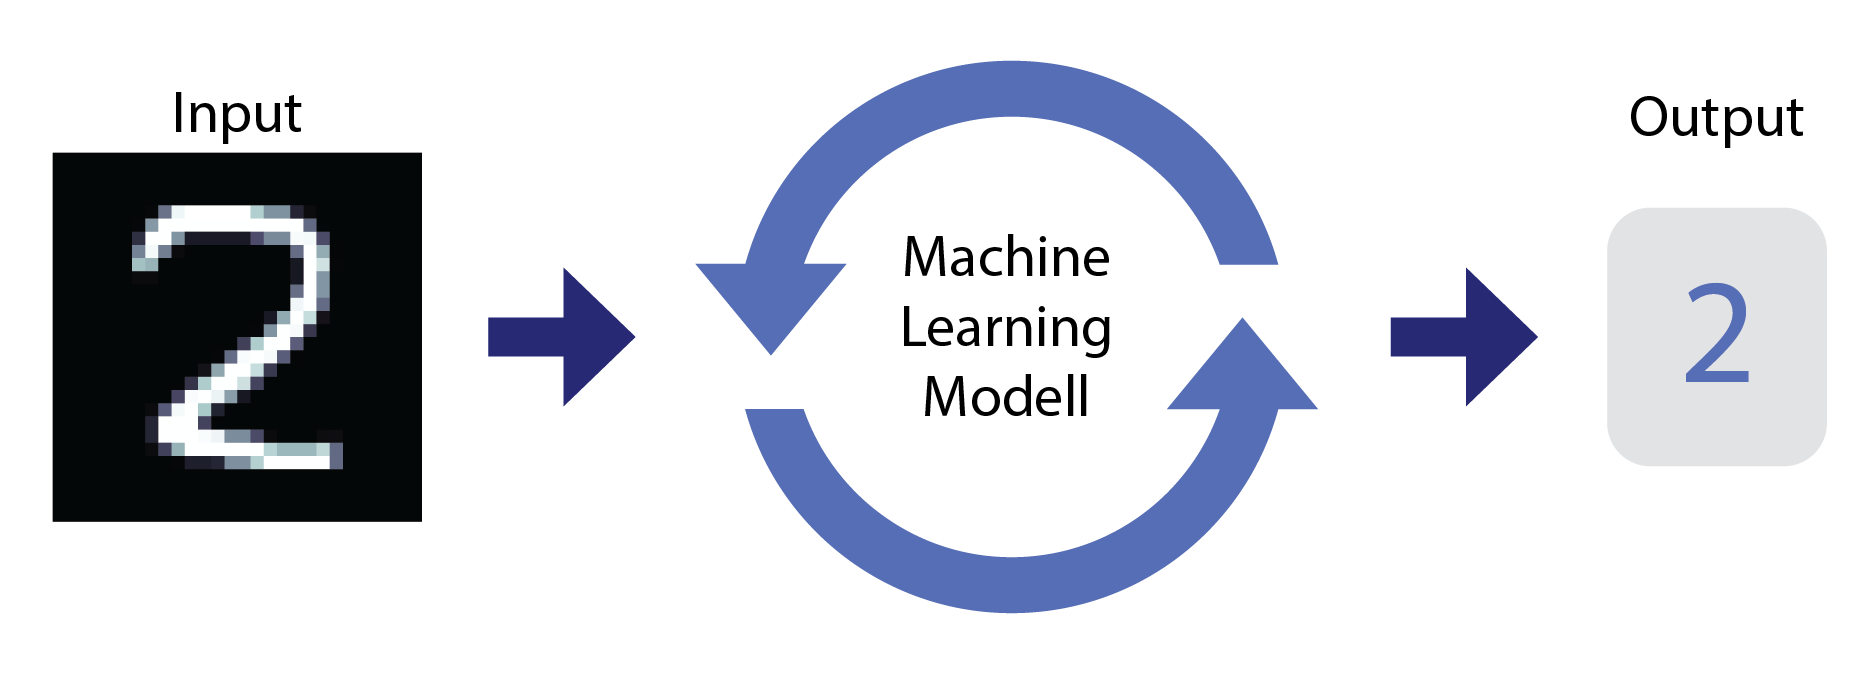
\includegraphics[width=\textwidth]{images/theorie/rec-maschine.png}
    \caption{Erkennung von handgeschriebenen Zahlen durch ein Machine Learning Modell (eigene Abbildung)}
    \label{fig:rec-maschine}
\end{figure}
%todo caption, format

Machine Learning Modelle, die das Beispielproblem lösen, basieren üblicherweise
auf Supervised Learning. Das ist ein Teilbereich von Machine Learning, wobei das
Machine Learning Modell aus Rückmeldungen der korrekten Beurteilung, der
Zielvariable, als Reaktion auf ihre eigenen Beurteilungen lernt
\cite{noauthor_was_nodate-1}. Die Zielvariable muss dabei im Voraus für jeden
Datenpunkt in den analysierten Daten durch einen Menschen festgelegt sein
\cite{trahasich_31_2020}. Ausgedrückt durch den Fachbegriff müssen die Daten
labeled sein \cite{noauthor_21_nodate}. Weitere Teilbereiche von Machine
Learning sind Unsupervised Learning und Reinforcement Learning
\cite{arora_supervised_2020}. Beachte \nameref{chap:t_rl} für eine ausgeprägtere
Einführung in Reinforcement Learning.
% TODO: Quellen Referenz?

Machine Learning Modelle sind hauptsächlich in der programmiersprache Python
implementiert \cite{sadie_bennett_why_2019}. Dabei werden häufig Tensorflow und Keras
verwendet. Tensorflow ist ein Machine Learning Framework
\cite{noauthor_tensorflow_nodate}. Das bedeutet, dass Tensorflow fertige
Funktionen und Algorithmen bereitstellt, die für Machine Learning Modelle nötig
sind. Keras ist ein weiteres Machine Learning Framework, das selbst mit
Tensorflow funktioniert.


\subsection{Funktionsweise eines Machine Learning Modelles}\label{sub:t_ml_func}
Dieser Abschnitt erklärt die Funktionsweise eines Machine Learning Modelles,
basierend auf dem Beispielproblem aus dem letzten Abschnitt (siehe\nameref{chap:t_ml}). 

Bei den Daten, die das Machine Learning Modell analysiert handelt es sich in
diesem Fall um das MNIST Datenset \cite{noauthor_mnist_nodate}. Dieses Datenset
wurde vom NIST (National Institute of Standards and Technology) in Amerika
veröffentlicht und beinhaltet $70'000$ Bilder von handgeschriebenen Zahlen
\cite{noauthor_emnist_2017}. Jedes Bild hat eine Auflösung von $28\times28$
Pixeln (siehe \autoref{fig:mnist-beispiele}).

% Bild: MNIST Beispiele
\begin{figure}[!ht]
    \centering
    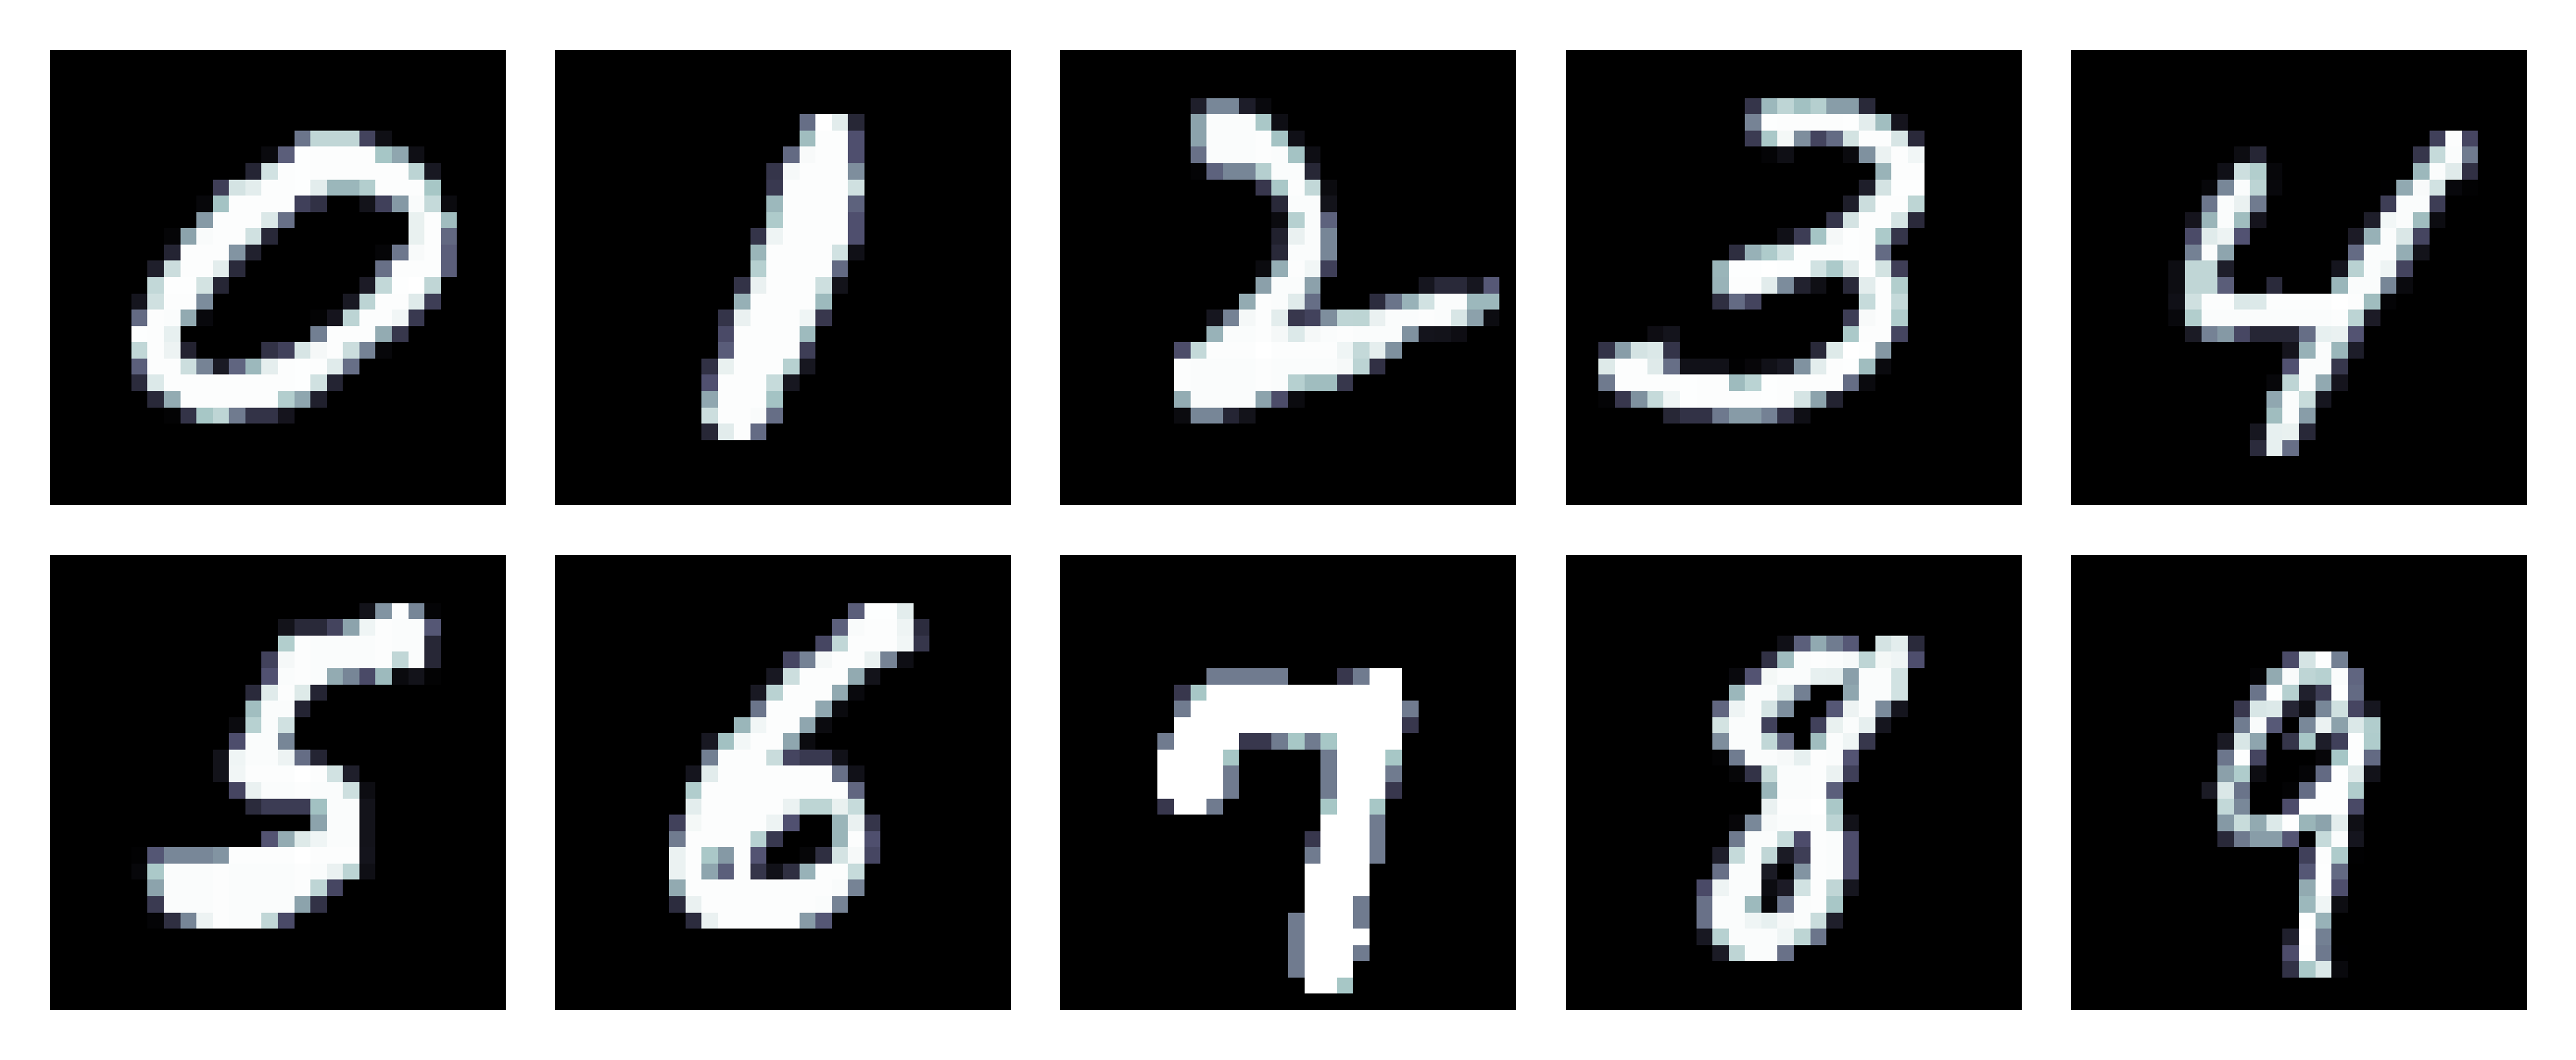
\includegraphics[width=\textwidth]{images/theorie/mnist-beispiele.png}
    \caption{Beispiele aus dem MNIST Datenset (Eigene Abbildung)}
    \label{fig:mnist-beispiele}
\end{figure}
%todo caption, format


                
Ein Machine Learning Modell durchläuft ein Training gefolgt von einer Testphase
\cite{noauthor_training_nodate}. Während dem Training erlernt das Modell die
Mustererkennung, um verlässliche Aussagen zu den Daten der Eingabe zu treffen.
Die Testphase misst die Genauigkeit des Modelles, also die Wahrscheinlichkeit,
mit der das Modell die richige Lösung zur Eingabe liefert. Nur in den seltensten
Fällen erreicht diese Genauigkeit $100\%$. Das Modell garantiert somit nicht die
richtige Lösung. Das Machine Learning Modell erlert die Mustererkennung während
dem Training durch die Analyse von Trainingsdaten aus einem Datenset. Das Modell
gibt zu jedem Datenpunkt die Beurteilung, um welche Zahl es sich handelt. Das
Datenset ist labeled (siehe \nameref{chap:t_ml}). Falls die Beurteilung des
Modelles nicht mit der bekannten, korrekten Lösung übereinstimmt, passt sich das
Modell automatisch an. Dadurch soll die Beurteilungen für zukünftige Datenpunkte
genauer werden. Die Testphase misst die Genauigkeit des Modelles auf Testdaten.
Die Testdaten bestehen aus Datenpunkten, die in den Trainingsdaten nicht
enthalten sind.

Zusammengefasst kann ein Machine Learning Modell Daten Beurteilen und sich
selbst Anpassen, um die Beurteilungen zu verbessern. Künstliche Neuronale Netze
(siehe \nameref{sub:t_ml_nn}) umfassen diese Funktionalität, und finden daher in
Machine Learning Modellen Anwendung.


\subsection{Hyperparameter}\label{sub:t_ml_hyper}
Machine Learning Modelle umfassen verschiedene Hyperparameter. Diese beschreiben
unter anderem wie lange das Training läuft oder wie stark sich das Modell nach
einer falschen Beurteilung anpasst. Diese Hyperparameter beeinflussen das
Lernverhalten des Modelles \cite{nyuytiymbiy_parameters_2022}, aber ihr optimaler Wert ist im
Voraus nicht bekannt.

Hyperparameter können unter anderem durch den Baysian Optimization Algorithmus
optimiert werden \cite{agnihotri_exploring_2020}\cite{paretos_bayesian_2021}.
Dieser Algorithmus versucht, den Output einer Black Box Funktion zu maximieren
oder zu minimieren \cite[S. 15]{garnett_bayesian_nodate}. Eine Black Box ist ein
häufig komplexes System, dessen inneren Vorgänge nicht betrachtet werden
\cite{noauthor_black_2021}. Bei einer Blackbox Funktion ist folglich der Input
und der Output bekannt, während die Verarbeitung des Inputs zum Output nicht
betrachtet wird (siehe \autoref{fig:blackbox}).
% TODO: Stimmen ersten beiden Quellen?

%bild Blackbox
\begin{figure}[!ht]
    \centering
    \includegraphics[width=\textwidth-2cm]{images/theorie/blackbox.png}
    \caption{Prinzip einer Black Box Funktion \cite{noauthor_fileblackboxsvg_nodate}}
    \label{fig:blackbox}
\end{figure}
%todo caption, format


Machine Learning Modelle werden häufig als Black Box Funktionen angesehen, da
das Training mit hohem rechnerischen Aufwand verbunden ist, wodurch die genauen
Vorgänge durch einen aussenstehenden Betrachter nicht oder nur schwer erfassbar
sind \cite{robbins_machine_2017}. Um ein Machine Learning Modell als eine BlackBox Funktion für
den Baysian Optimization Algorithmus zu verwenden, werden die zu optimierenden
Hyperparameter als Input und eine Zielvariable als Output definiert. Die
Zielvarible des Outputs entspricht dabei einem Wert, der die Leistung des
Modelles widerspiegelt und durch den Algorithmus maximiert werden soll. Ein
Beispiel für die Zielvarible wäre die Genauigkeit des Machine Learning Modelles
(siehe \nameref{sub:t_ml_func}). Die inneren Vorgänge in der BlackBox Funktion
entsprechen in diesem Fall einem Training des Modelles.

Der Baysian Optimization Algorithmus kann bis zu 20 Hyperparameter zuverlässig
optimieren \cite{moriconi_high-dimensional_2020}. Der Algorithmus führt die Blackbox Funktion für eine
bestimmte Anzahl Iterationen mit jeweils verschiedenen Parametern durch. Die
Wahl der Parameter basiert dabei auf Bayes' Theorem \cite[S. 7]{garnett_bayesian_nodate}.
Diejenigen Parameter, die den höchsten gefundenen Wert der Zielvariable
auslösen, werden gespeichert.


\subsection{künstliche neuronale Netze}\label{sub:t_ml_nn} Ein neuronales Netz
ist, im biologischen Sinne, "eine beliebige Anzahl Neuronen, die miteinander
Verbunden sind" \cite{noauthor_neuronales_2021}. Ein Beispiel für ein neuronales
Netz ist das menschliche Gehirn. Künstliche Neuronale Netze modellieren
biologische neuronale Netze in der Form von Programmcode
\cite{noauthor_artificial_nodate}. Diese Arbeit behandelt künstliche neuronale
Netze, nicht aber biologische. Somit handelt es sich bei jedem erwähnten
neuronalen Netz, um ein künstliches neuronales Netz.

Der Grundbaustein eines neuronalen Netzes ist das Neuron. Im Modell stellt das
Neuron ein Objekt dar, das eine beliebiege Anzahl Inputs, aber nur einen Output
hat (siehe \autoref{fig:neuron}) \cite{pramoditha_concept_2021}. Input und Output
sind hierbei rationale Zahlen. Die Ausgabe des Neurons ist im einfachsten
Modell, dem Perzeptron Neuron, grundsätzlich entweder 0 oder 1. Die Ausgabe ist
1, wenn die Summe der Eingaben einen vorgegebenen Wert, den \emph{Threshold},
überschreitet. Ansonsten ist die Ausgabe gleich 0. Jede Eingabe hat ein
\emph{Gewicht}, das einer rationalen Zahl entspricht. Vor der Addition der
Inputs wird jeder Input mit seinem Gewicht multipliziert.  Die Grösse des
Gewichts bestimmt somit den Einfluss der zugehörigen Eingabe auf die Ausgabe des
Neurons. \cite{nielsen_neural_2015}\cite{simplilearn_what_2021}

% Bild Neuron
\begin{figure}[!ht]
    \centering
    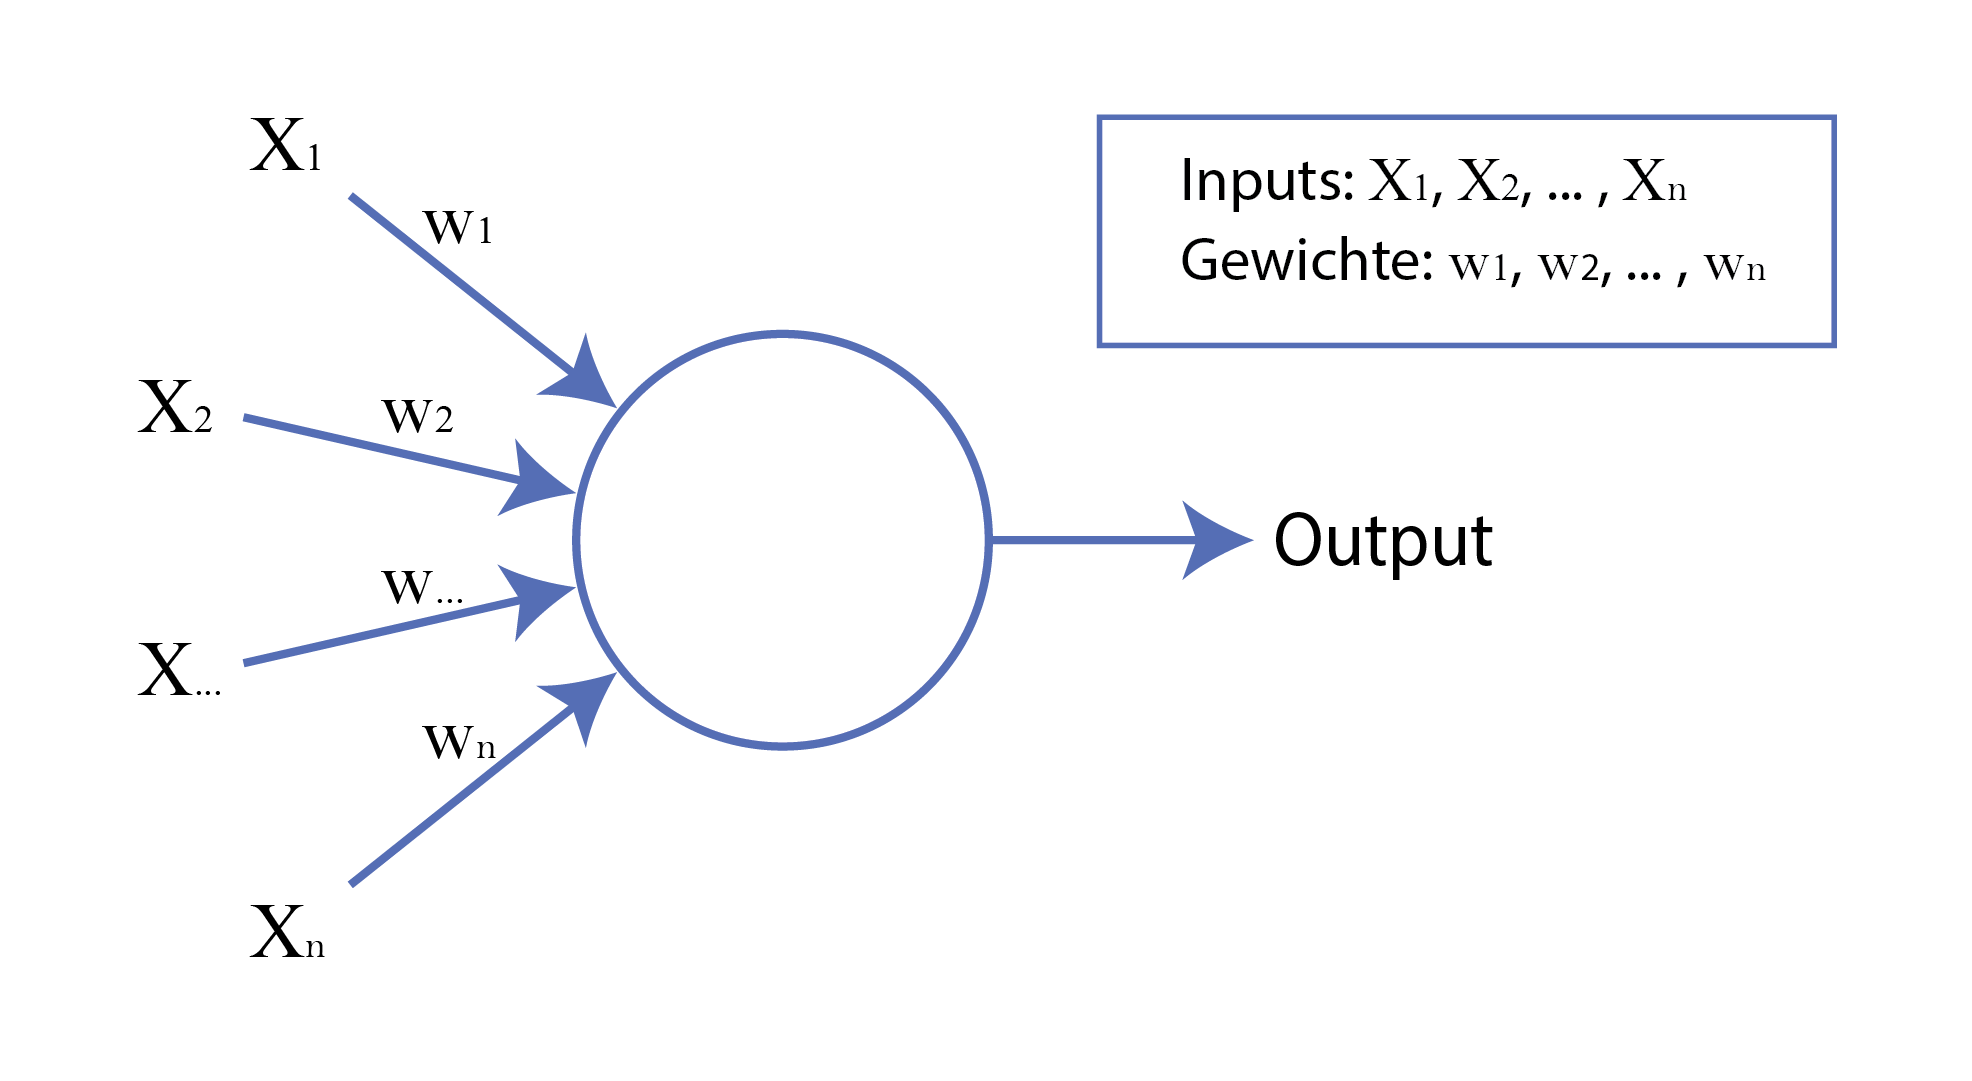
\includegraphics[width=\textwidth]{images/theorie/neuron.png}
    \caption{Perzeptron Neuron (eigene Abbildung)}
    \label{fig:neuron}
\end{figure}
%todo caption, format

Neuronale Netze in Machine Learning Modellen verwenden kompliziertere Neuronen
als das Perzeptron Neuron, wie zum Beispiel das Sigmoid-Neuron. Die Neuronen
unterscheiden sich in ihrer Activation Function und somit im Verhalten ihres
Outputs \cite{pragati_baheti_activation_2022}. So nimmt der Output im Sigmoid Neuron
beispielsweise auch Werte zwischen $0$ und $1$ an in einem stetigen Übergang
zwischen den beiden Grenzen (siehe \autoref{fig:percep-v-sig}) \cite{kumar_sigmoid_2019}.

%Bild sigmoid vs perceptro
\begin{figure}[!ht]
    \centering
    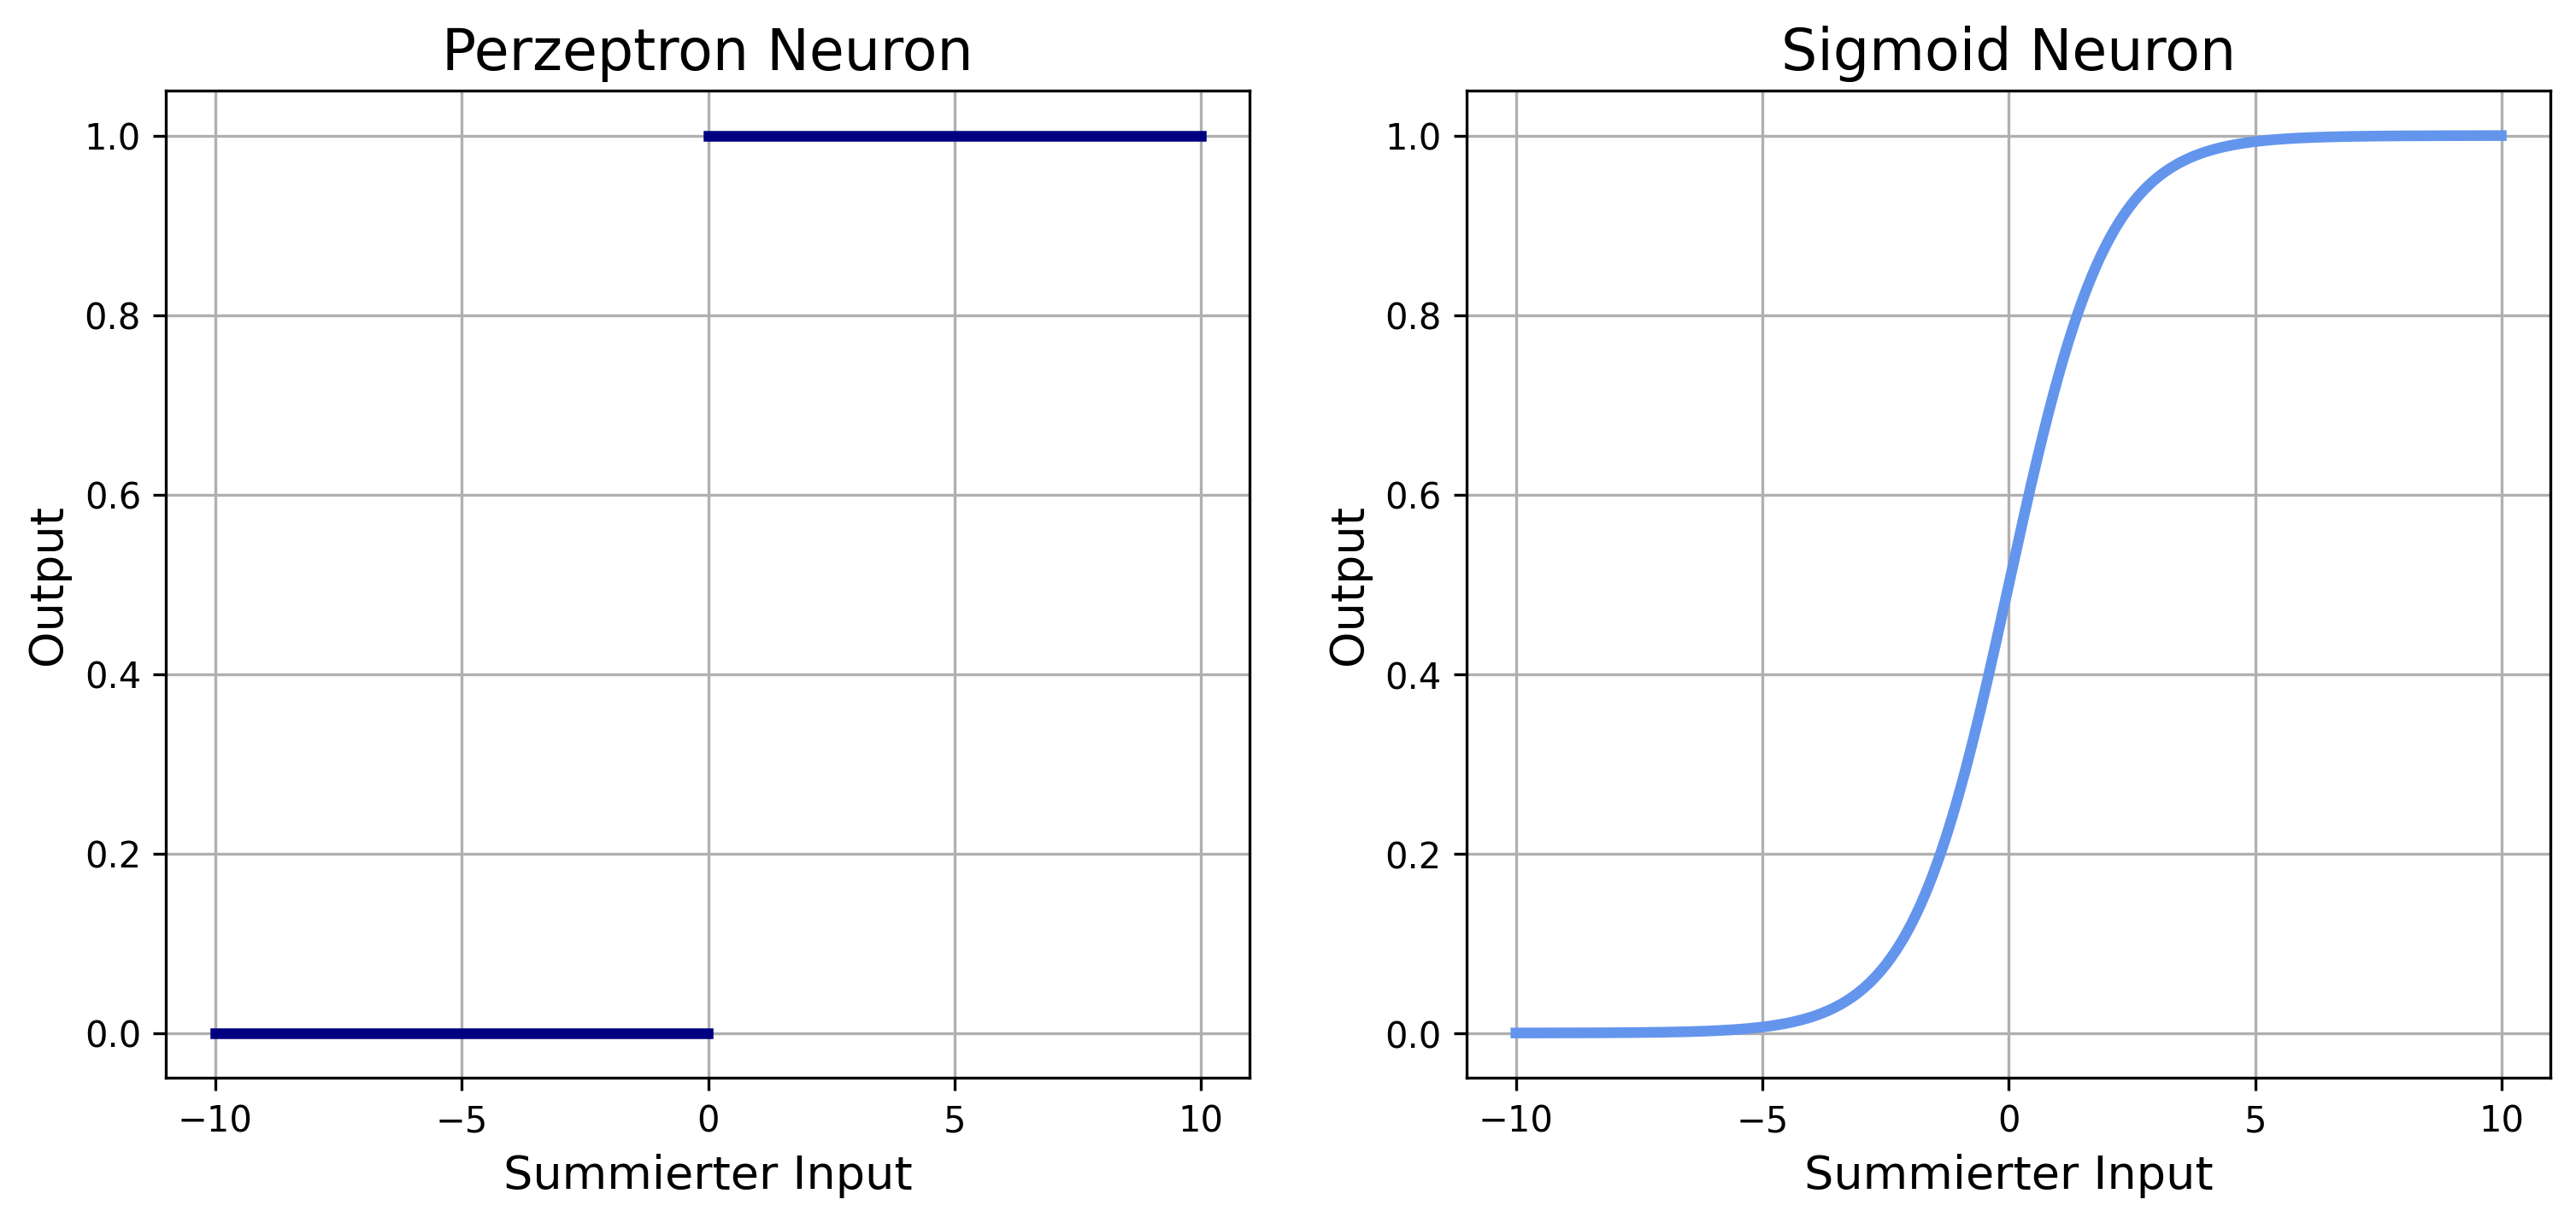
\includegraphics[width=\textwidth]{images/theorie/percep-v-sig.png}
    \caption{Vergleich des Outputs eines Perzeptron Neurons und eines Sigmoid Neurons (eigene Abbildung)}
    \label{fig:percep-v-sig}
\end{figure}
%todo caption, format

Neuronale Netze sind Verbindungen dieser Neuronen. Dabei dient der Output eines
Neurons als Input in ein anderes Neuron. Der Output eines Neurons kann gleich
für mehrere Neuronen ein Input sein. Die Neuronen sind in \emph{Layers} geordnet
(siehe autoref{layers}). Neuronale Netze haben mindestens einen \emph{Input
Layer} und einen \emph{Output Layer}
\cite{nielsen_neural_2015}\cite{ognjanovski_everything_2020}. Der Input Layer
umfasst die Daten, zu dem das neuronale Netz eine Beurteilung liefern soll. Im
Beispielproblem (siehe \nameref{chap:t_ml}) bestände die Eingabe-Ebene aus
$28\times28$ Neuronen, wobei jedes Neuron die Graustufe (durch einen Wert von
$0$ bis $255$) eines Pixels im Bild beschreibt. Der Input ist in diesem Fall
zweidimensional. Die Dimensionen sind allerdings flexibel. Die Output Layer
besteht im Beispiel aus $10$ Neuronen, wobei jedes Neuron einer Beurteilung
entspricht (das fünfte Neuron beschreibt zum Beispiel die Ziffer Fünf als
Beurteilung). Dasjenige Neuron mit dem höchsten Output entspricht der
Beurteilung des neuronalen Netzes. (siehe \autoref{fig:layers}).

%Bild Layers
\begin{figure}[!ht]
    \centering
    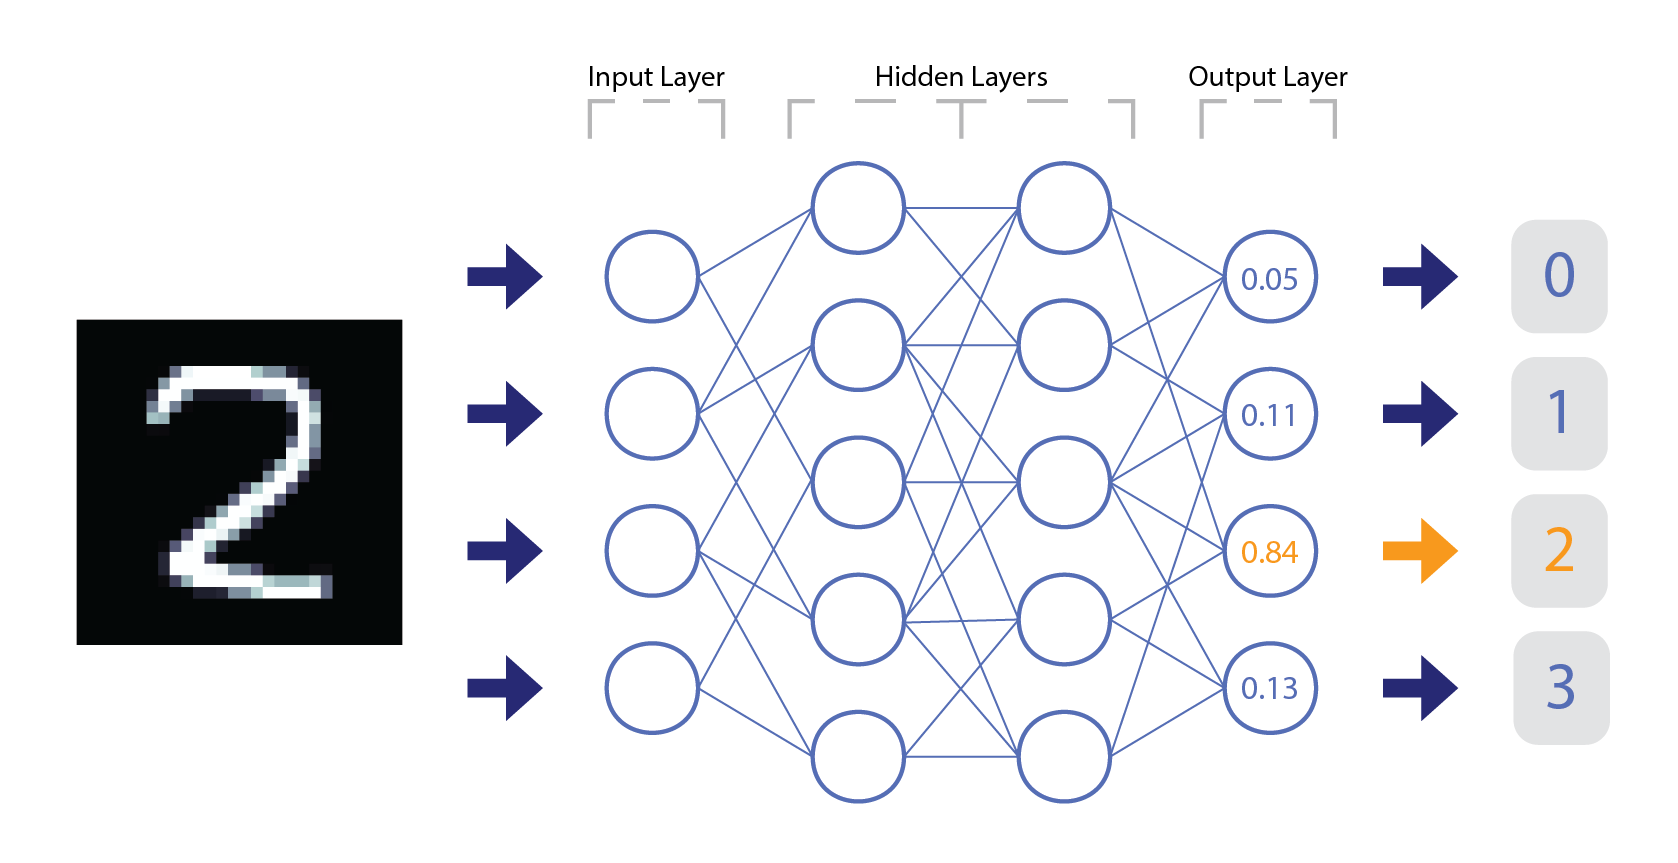
\includegraphics[width=\textwidth]{images/theorie/layers.png}
    \caption{Neuronales Netz mit beschrifteten Layers (eigene Abbildung)}
    \label{fig:layers}
\end{figure}
%todo caption, format

Zwischen dem Input Layer und dem Output Layer kann es weitere \emph{Hidden
Layers} geben \cite{malik_what_2019}. Es gibt verschiedene Arten von Hidden
Layers, die verschidene Funktionen haben. Zwei der meist verwendeten Layers sind
Fully Connected (Dense) Layers und Convolutional Layers
\cite{unzueta_convolutional_2022}. In Fully Connected Layers dient jedes Neuron
als Input für jedes Neuron in der nächsten Layer. In Convolutional Layers trifft
das nicht zu (siehe \autoref{fig:conv-v-dens}). Die Funktion von Convolutional
Layers beinhaltet es, wichtige Merkmale aus dem Input hervorzuheben
\cite{deshpande_beginners_nodate}. Concatenation Layers
\cite{jayawardana_concatenating_2021} sind eine weitere Form von hidden Layers,
die zwei verschiedene Layers als Input haben und diese somit verbinden. Machine
Learning Modelle werden ab mehr als einer Hidden Layer als Deep Learning Modelle
bezeichnet \cite{jan-dirk_kranz_deep_2019}.

%Bilder conv-v-dens dens-v-conv
%file:///C:/Users/robin/Zotero/storage/PAZJPWRZ/convolutional-layers-vs-fully-connected-layers-364f05ab460b.html
\begin{figure}[!ht]
    \centering
    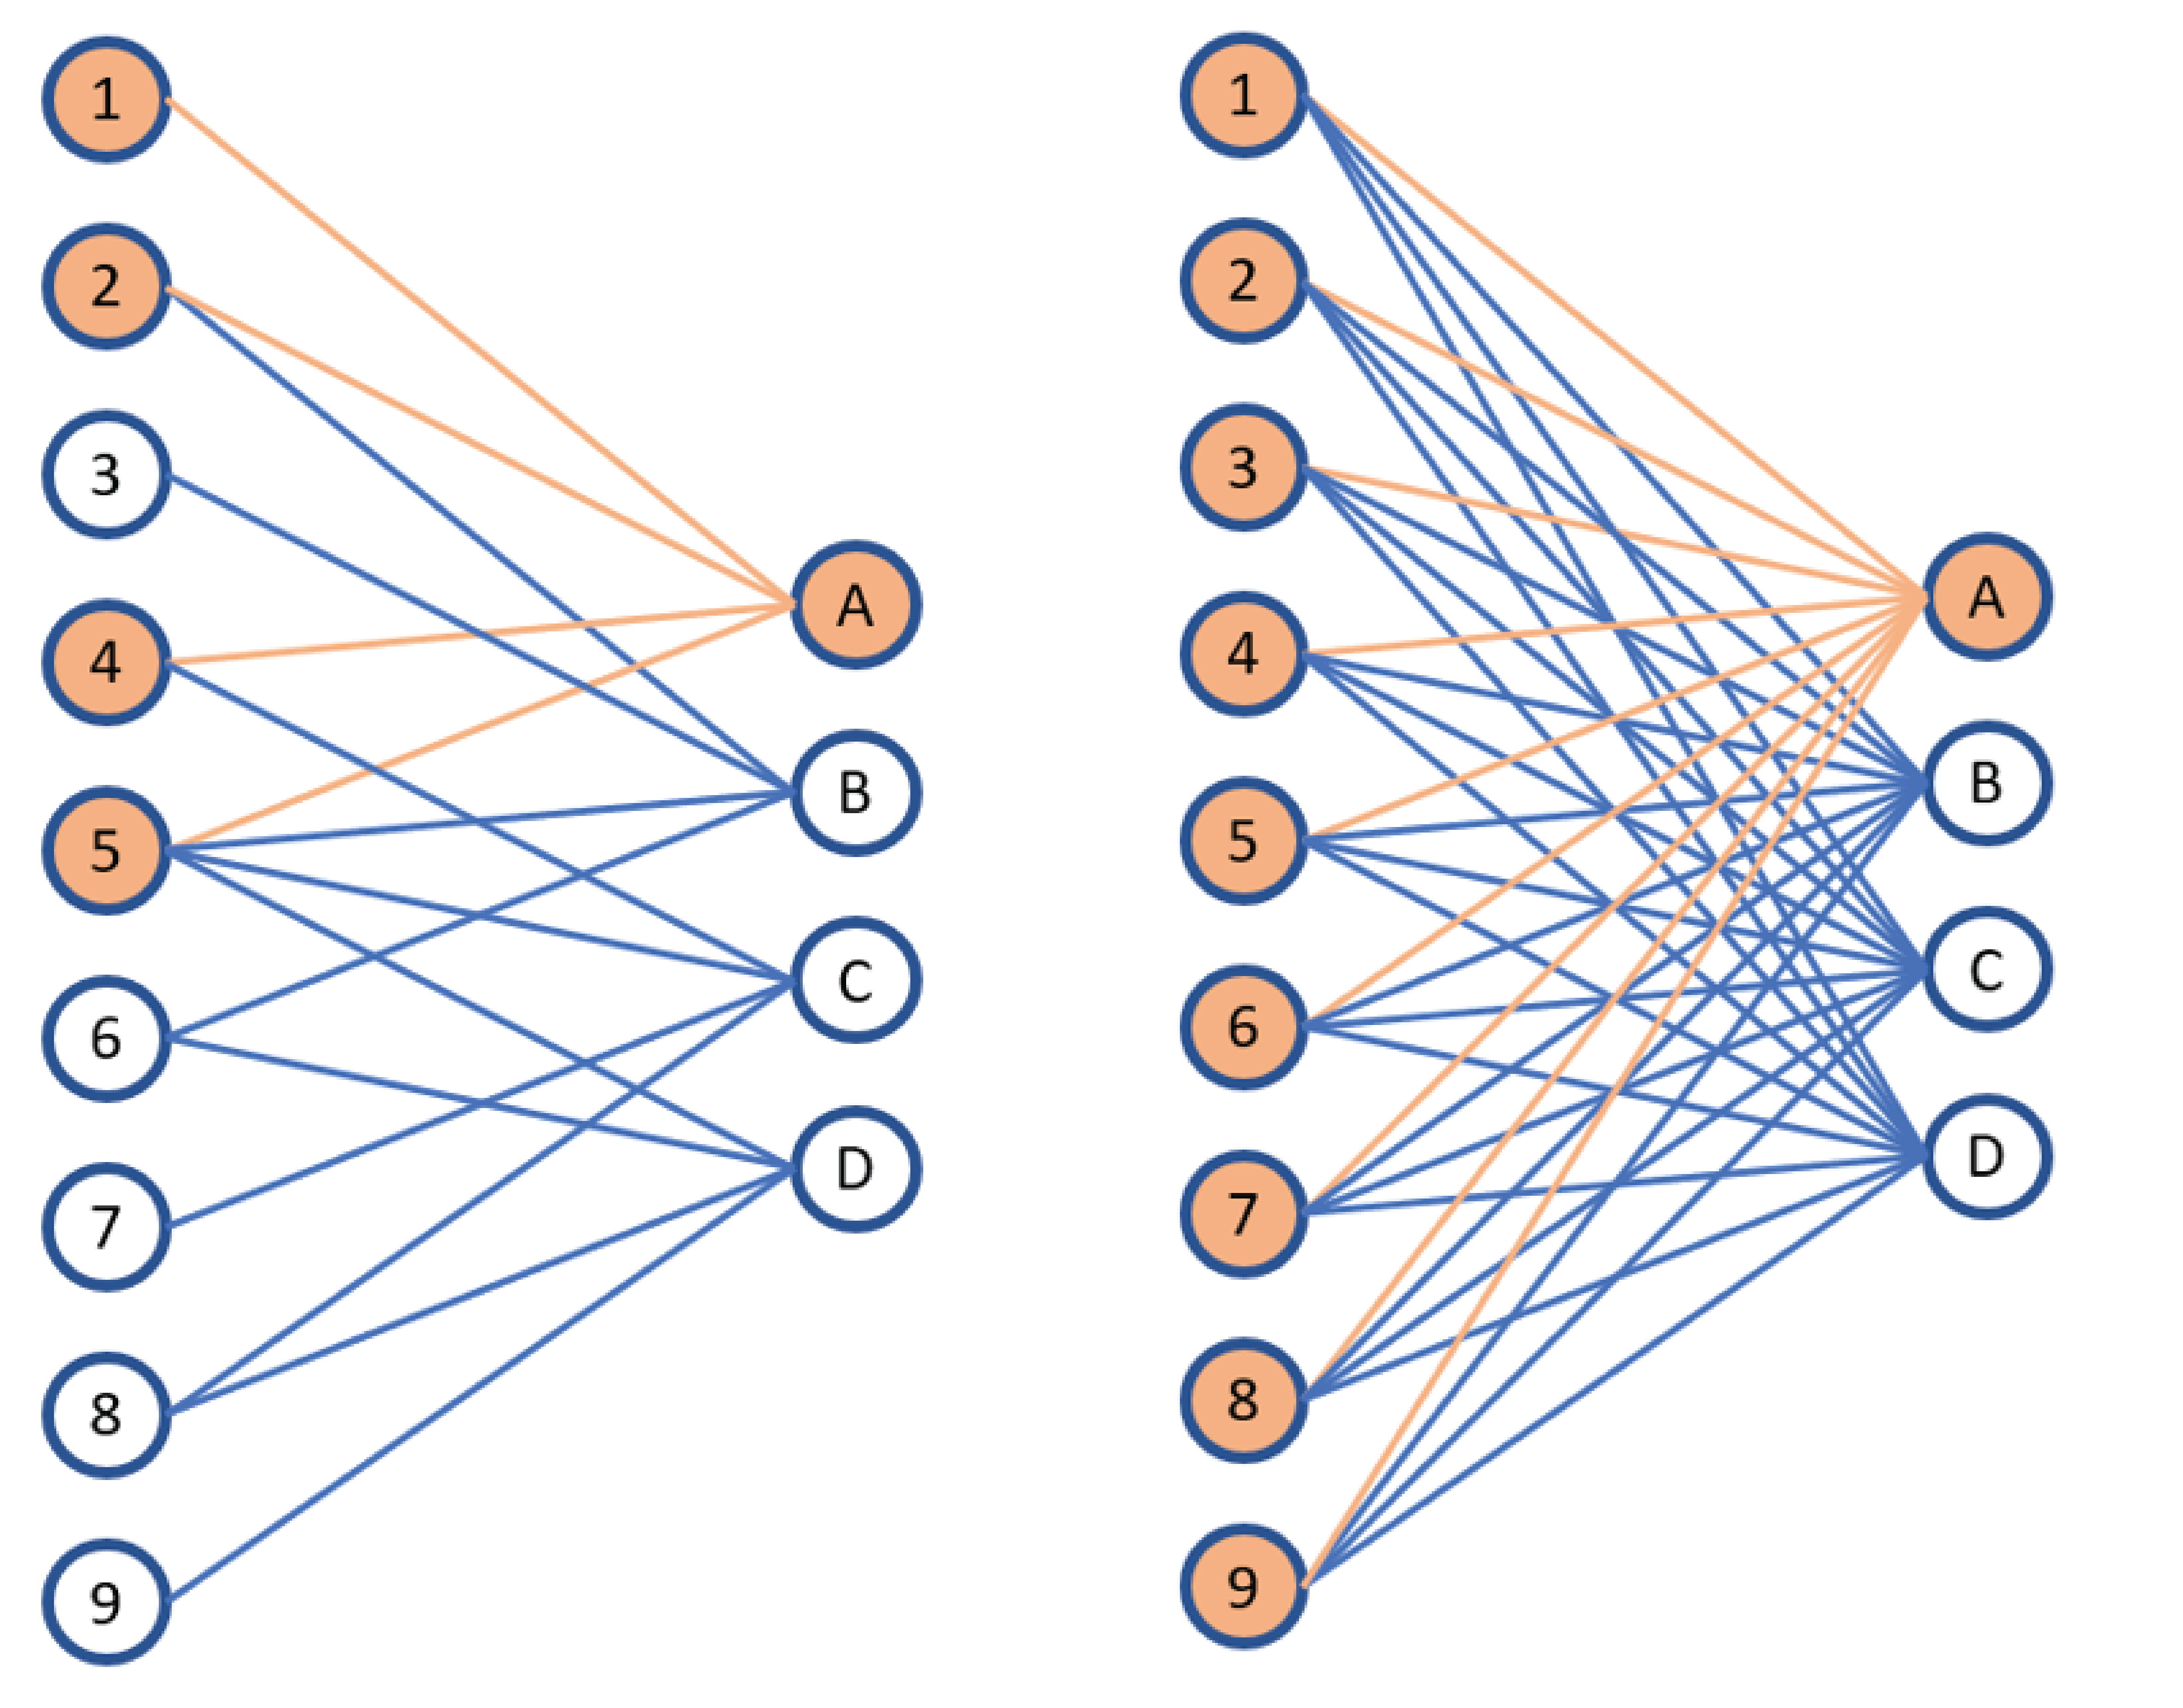
\includegraphics[width=\textwidth]{images/theorie/conv-v-dens.png}
    \caption{Vergleich zwischen Convolutional Layers (links) und Fully Connected Layers (rechts) \cite{unzueta_convolutional_2022}}
    \label{fig:conv-v-dens}
\end{figure}
%todo caption, format

Ein Machine Learning Modell passt während dem Training (siehe
\nameref{sub:t_ml_func}) einzelne Gewichte im neuronalen Netz an, in der Hoffnung,
dass die Genauigkeit der Beurteilung mit den angepassten Gewichten grösser
ist. Die genaue Anpassung erfolgt in den meisten Machine Learning Modellen durch
den Backpropagation Algorithmus
\cite{ognjanovski_everything_2020}\cite{david_e_rumelhart_learning_nodate}.

\section{Reinforcement Learning}\label{chap:t_rl}
Reinforcement Learning bedeutet Lernen durch Interaktion mit einer Umgebung.
\cite{osinski_what_2018}. Genauer gesagt soll ein Machine Learning Modell durch
Rückmeldungen und Beobachtungen aus einer Umgebung ein bestimmtes Verhalten
erlernen.

Reinforcement Learning Modelle führen somit die Umgebung ein. Anders als bei
Supervised Learning und Unsupervised Learning (siehe \nameref{chap:t_ml}) sind
die Daten, aus denen das Modell lernen soll, im Voraus nicht bekannt.
Reinforcement Learning Modelle trainieren somit nicht auf der Grundlage eines
Datensets. Das liegt in der Natur der Umgebung, die häufig zu viele verschiedene
Zustände einnehmen kann, als dass diese in einem Datenset gesammelt werden
könnten. Ein Machine Learning Modell kann trotzdem aus einer Umgebung lernen,
indem es selbst mit dieser interagiert und dadurch Erfahrung sammelt.
\cite{piyush_verma_what_2021}

Als Beispiel kann die echte Welt als eine Umgebung angesehen werden. Der Mensch
wäre in diesem Fall das Reinforcement Learning Modell. Der Mensch lernt die
Eigenschaften seiner Umgebung durch Interaktionen mit dieser kennen.
Beispielsweise lernt ein Mensch die Schwerkraft durch das Hinfallen kennen.
Durch diese Erfahrungen kann der Mensch ein gewisses Verhalten, zum Beispiel das
Laufen, erlernen. Reinforcement Learning Modelle imitieren dieses Lernverhalten.
So verwendet die Robotik häufig Reinforcement Learning, um einen Roboter laufen
zu lassen. Die Umgebung, mit der das Reinforcement Learning Modell lernt, ist
dabei häufig nicht echt, sondern simuliert.

\subsection{Aufbau und Funktionsweise}\label{sub:t_rl_func}
Dieser Abschnitt umfasst eine genauere Erklärung eines Reinforcement Learning
Modelles, in diesem Fall Deep Q-Learning, unter der Verwendung der korrekten
Fachbegriffe.

Ein Reinforcement Learning Modell umfasst eine \emph{Umgebung} und einen
\emph{Agent}. Der Agent ist dasjenige Element in der Umgebung, welches mit
dieser interagiert und daraus lernt \cite[S. 53]{sutton_reinforcement_2014}. Die
Umgebung verändert sich in Zeitschritten, genannt \emph{Steps}. In jedem Step
führt der Agent eine \emph{Action} aus, die die Umgebung beeinflusst. Die
Entscheidung, welche Action der Agent ausführt, basiert auf einer
\emph{Observation} \cite[S. 2]{mnih_playing_2013} der Umgebung. Die
Observation umfasst alle Daten der Umgebung, die für die Entscheidung des Agents
relevant sind. Der Agent trifft seine Entscheidung auf der Basis eines
neuronalen Netzes (siehe \nameref{sub:t_ml_nn}). Der Input in dieses neuronale
Netz ist die Observation der Umgebung und der Output beschreibt die Action, die
der Agent ausführt. Jedes Neuron des Outputs beschreibt eine spezifische Action
des Agents. Der Agent kann somit nur eine feste Anzahl Actions ausführen. Alle
Actions zusammen werden \emph{Action-Space} \cite[S.
67]{sutton_reinforcement_2014} genannt. Jede Action im Action-Space besitzt
einen \emph{Q-Value}, der dem Output des zugehörigen Neurons entspricht. (siehe
\autoref{fig:reinforce-1}) \cite{wang_deep_2021} Die schlussendliche Entscheidung, welche
Action ausgeführt wird, basiert auf der \emph{Epsilon-Greedy} Strategie \cite[S.
34]{sutton_reinforcement_2014}. Diese Strategie sieht vor, dass die Entscheidung
mit einer Wahrscheinlichkeit von $\epsilon$ auf eine zufällige Action fällt.
Ansonsten fällt die Entscheidung auf diejenige Action mit dem höchsten Q-Value.
Der Agent erkundet die Umgebung durch die zufälligen Actions, die er teilweise
wählt. Der Agent wählt Actions, die er ansonsten nie wählen würde, und trifft
möglicherweise zufällig auf bessere Optionen für zukünftige Steps
\cite{rajendra_koppula_exploration_nodate}.

%bild reinforcement schema 1
\begin{figure}[!ht]
    \centering
    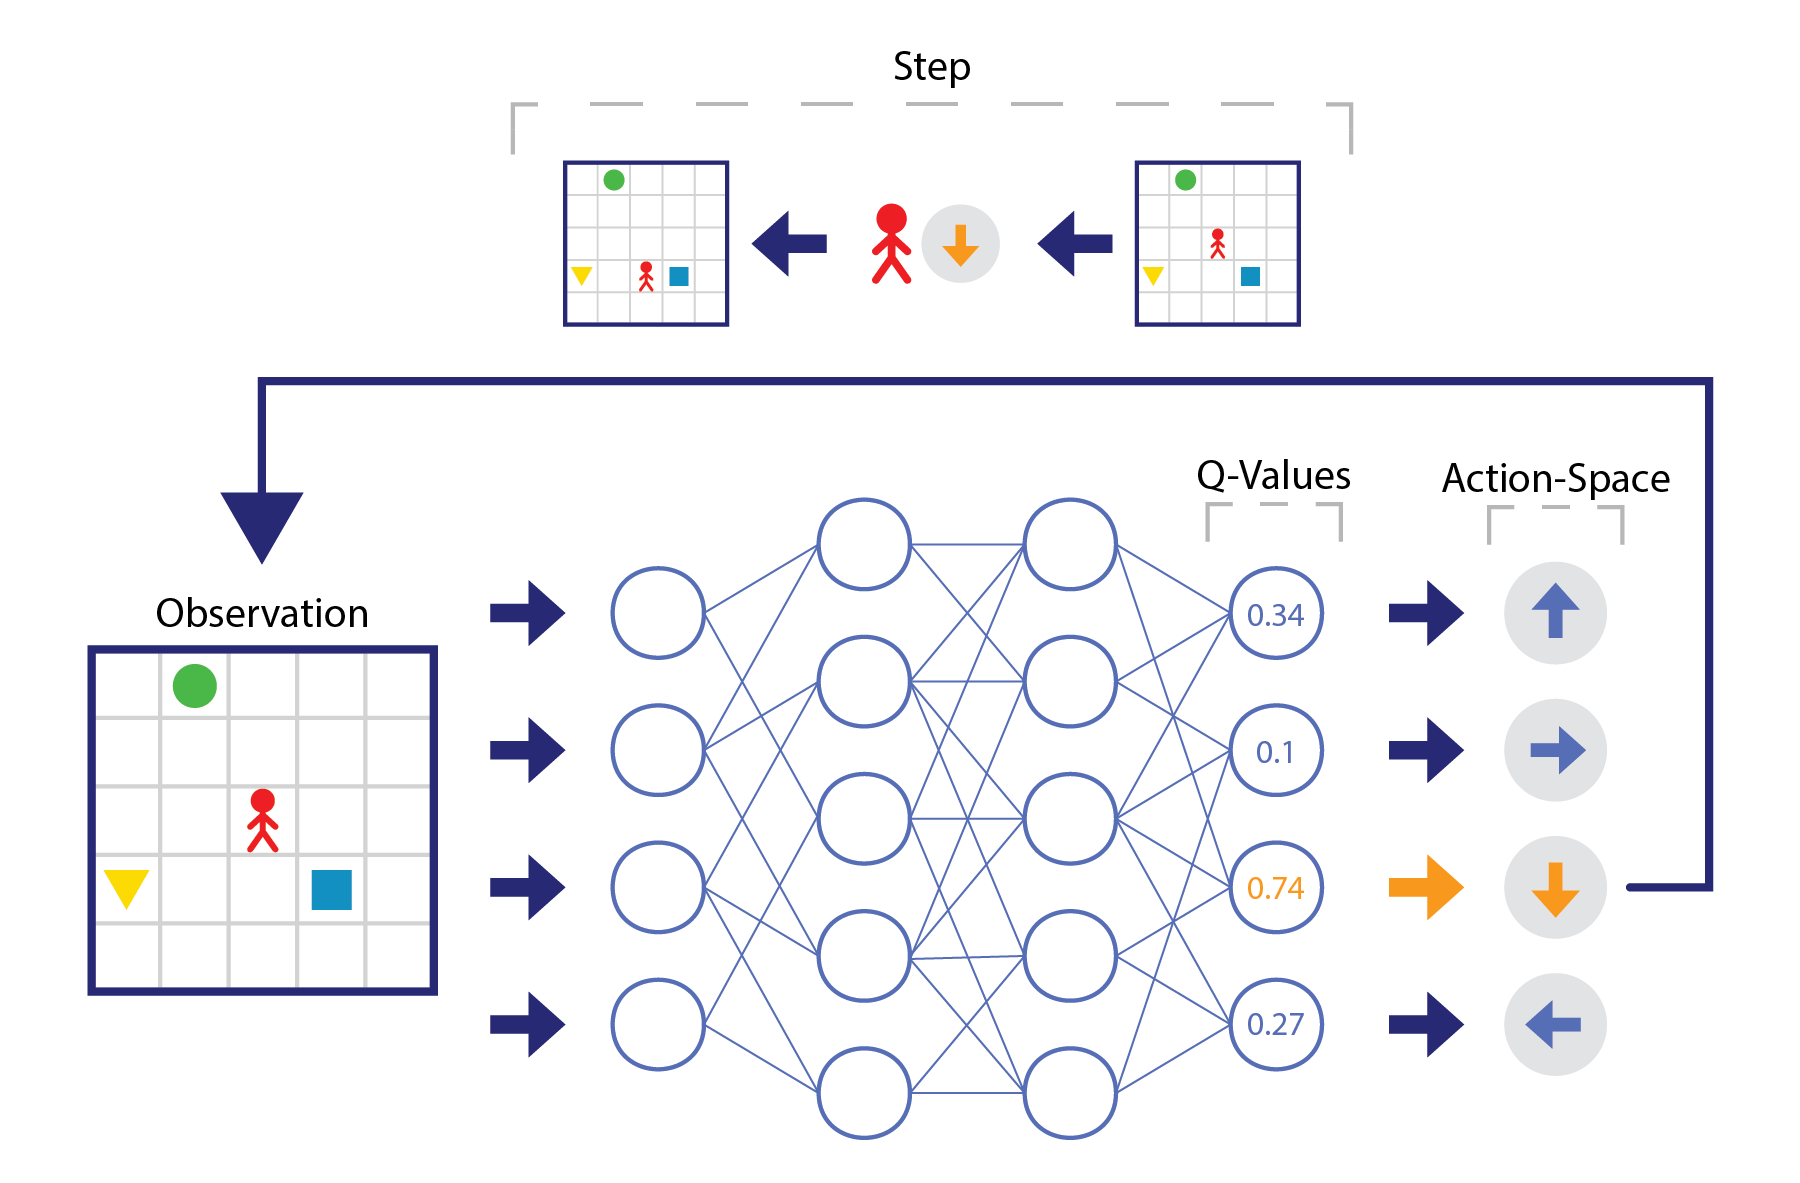
\includegraphics[width=\textwidth]{images/theorie/reinforce-1.png}
    \caption{Funktionsweise eines Reinforcement Learning Modelles (eigene Abbildung)}
    \label{fig:reinforce-1}
\end{figure}
%todo caption, format

Die Umgebung und somit auch der Agent werden durch die Actions des Agenten
beeinflusst. Dieser Einfluss wird durch die \emph{Reward-Function} gemessen. Die
Reward-Function gibt eine rationale Zahl, den \emph{Reward} aus \cite[S.
75]{sutton_reinforcement_2014}. Umso grösser der Reward, desto positiver ist der
Effekt auf die Umgebung und umgekehrt. Ein positiver Einfluss auf die Umgebung
durch eine Action ist so definiert, dass der Agent durch die Action das
gewünschte Verhalten vorzeigt. Die Reward-Function definiert, welches Verhalten
welchen Reward erzielt. Der Q-Value der gewählten Action wird mit dem Reward
(und dem maximalen Q-Value aus den nächsten möglichen Actions) addiert. Diese
Formel nennt sich Bellman-Gleichung \cite[S. 3]{mnih_playing_2013}. Der neue
Q-Value hat somit einen kleineren Wert, wenn der Reward negativ ist, und einen
grösseren Wert, wenn der Reward positiv ist. Die das neuronalen Netz wird
daraufhin so trainiert, dass der Output für das Neuron, dessen Action ausgeführt
wurde, näher am neu berechneten, besseren Q-Value ist (siehe \autoref{fig:reinforce-2}).
Der schlussendliche Effekt ist, dass Actions, die einen positiven Reward
auslösen, wahrscheinlicher gewählt werden, und umgekehrt Actions, die einen
negativen Rewards auslösen, unwahrscheinlicher gewählt werden. Der Agent
versucht insgesamt durch seine Actions einen möglichst hohen akkumulierten
Reward zu erzielen \cite[S. 57]{sutton_reinforcement_2014}. Der akkumulierte
Reward entsprich der Summe der Rewards aus jedem Step in einer Episode.

%bild reinforcement schema 2
\begin{figure}[!ht]
    \centering
    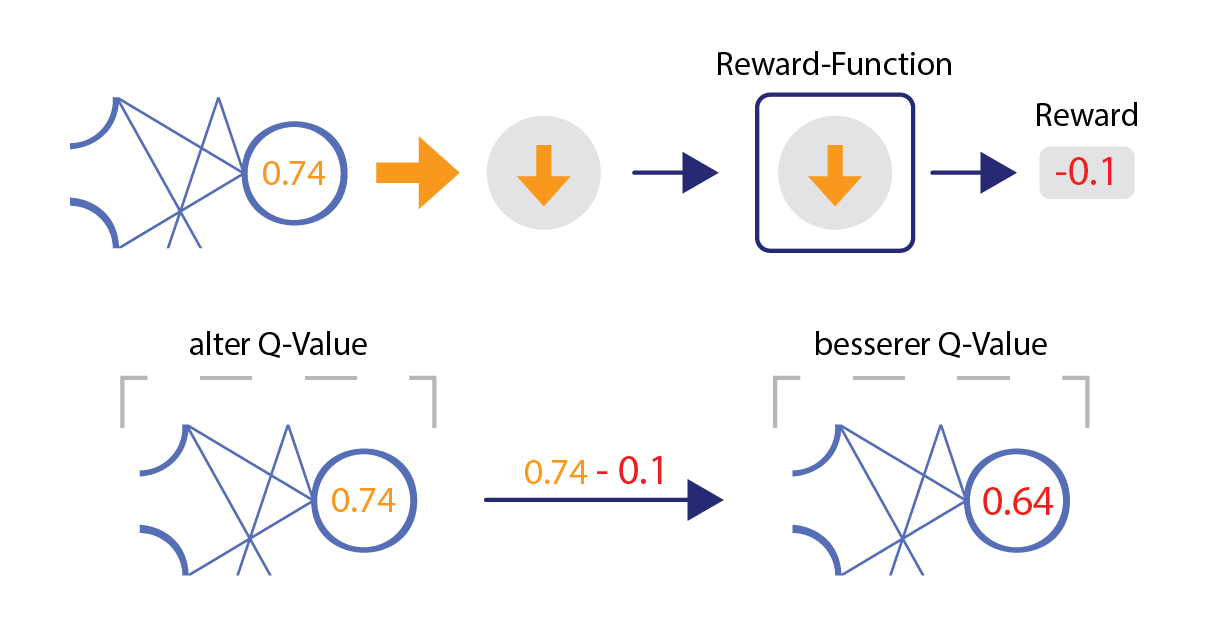
\includegraphics[width=\textwidth]{images/theorie/reinforce-2.png}
    \caption{Funktionsweise einer Reward-Function (eigene Abbildung)}
    \label{fig:reinforce-2}
\end{figure}
%todo caption, format

Das Training läuft in \emph{Episodes} \cite[S. 14]{sutton_reinforcement_2014}.
Eine Episode umfasst eine gewisse Anzahl Steps und am Anfang jeder Episode wird
die Umgebung in einen Startzustand zurückgesetzt. Die Resultate eines Steps
werden in dem \emph{Replay-Buffer} gespeichert. Dazu gehören die Observation der
Umgebung, die jeweiligen Actions und der jeweilige Reward. Der Replay-Buffer enthält Speicherplatz
für eine bestimmte Anzahl Steps. Während dem Training werden zufällige Steps aus
dem Replay-Buffer gewählt, auf die das neuronale Netz trainiert. Das neurnale
Netz trainiert also auf Daten aus der Vergangenheit der Umgebung und des Agents.
Diese Strategie nennt sich Experience Replay \cite[S. 5]{mnih_playing_2013}.
Ausserdem trainiert das neuronale Netz jeweils mit einem \emph{Batch} an Steps,
also mit einer gewissen Anzahl an Steps gleichzeitig. Der Replay-Buffer und der
Batch sichern zu, dass das neuronale Netz mit einer grossen Vielfalt an Steps
trainiert, was das Lernverhalten stabiler macht als ein chronologisches Training
auf einzelne Steps \cite{phd_how_2021}.


\section{Verwandte Arbeiten und Themen}\label{chap:t_ver} Das Nachzeichnen von
Strichbildern ist ein Teilbereich von dem Zeichnen allgemein. Es gibt
verschiedene Ansätze, um einen Computer zeichnen zu lassen. Ein häufiger Ansatz
ist \emph{Stroke-Based Rendering} \cite{hertzmann_stroke_2002}. Stroke-Based % TODO: Quelle?
Rendering ist das Zeichnen von Bilder durch das Platzieren von Elementen wie
Strichen. Beispiele für Arbeiten in diesem Bereich sind Strokenet
\cite{zheng2018strokenet} und ``Learning to Paint With Model-based Deep
Reinforcement Learning'' \cite{huang_learning_2019} Andere Ansätze simulieren
die Führung eines Stiftes. (siehe \autoref{fig:stroke-v-stift}) Ein Beispiel
dafür ist das Programm Doodle-SDQ \cite{zhou_learning_2018}. Doodle-SDQ
beschäftigt sich auch spezifischer mit dem Nachzeichnen von Strichbildern und
wird deswegen im nächsten Abschnitt weiter behandelt.

%bild strokebased vs stife
\begin{figure}[!ht]
    \centering
    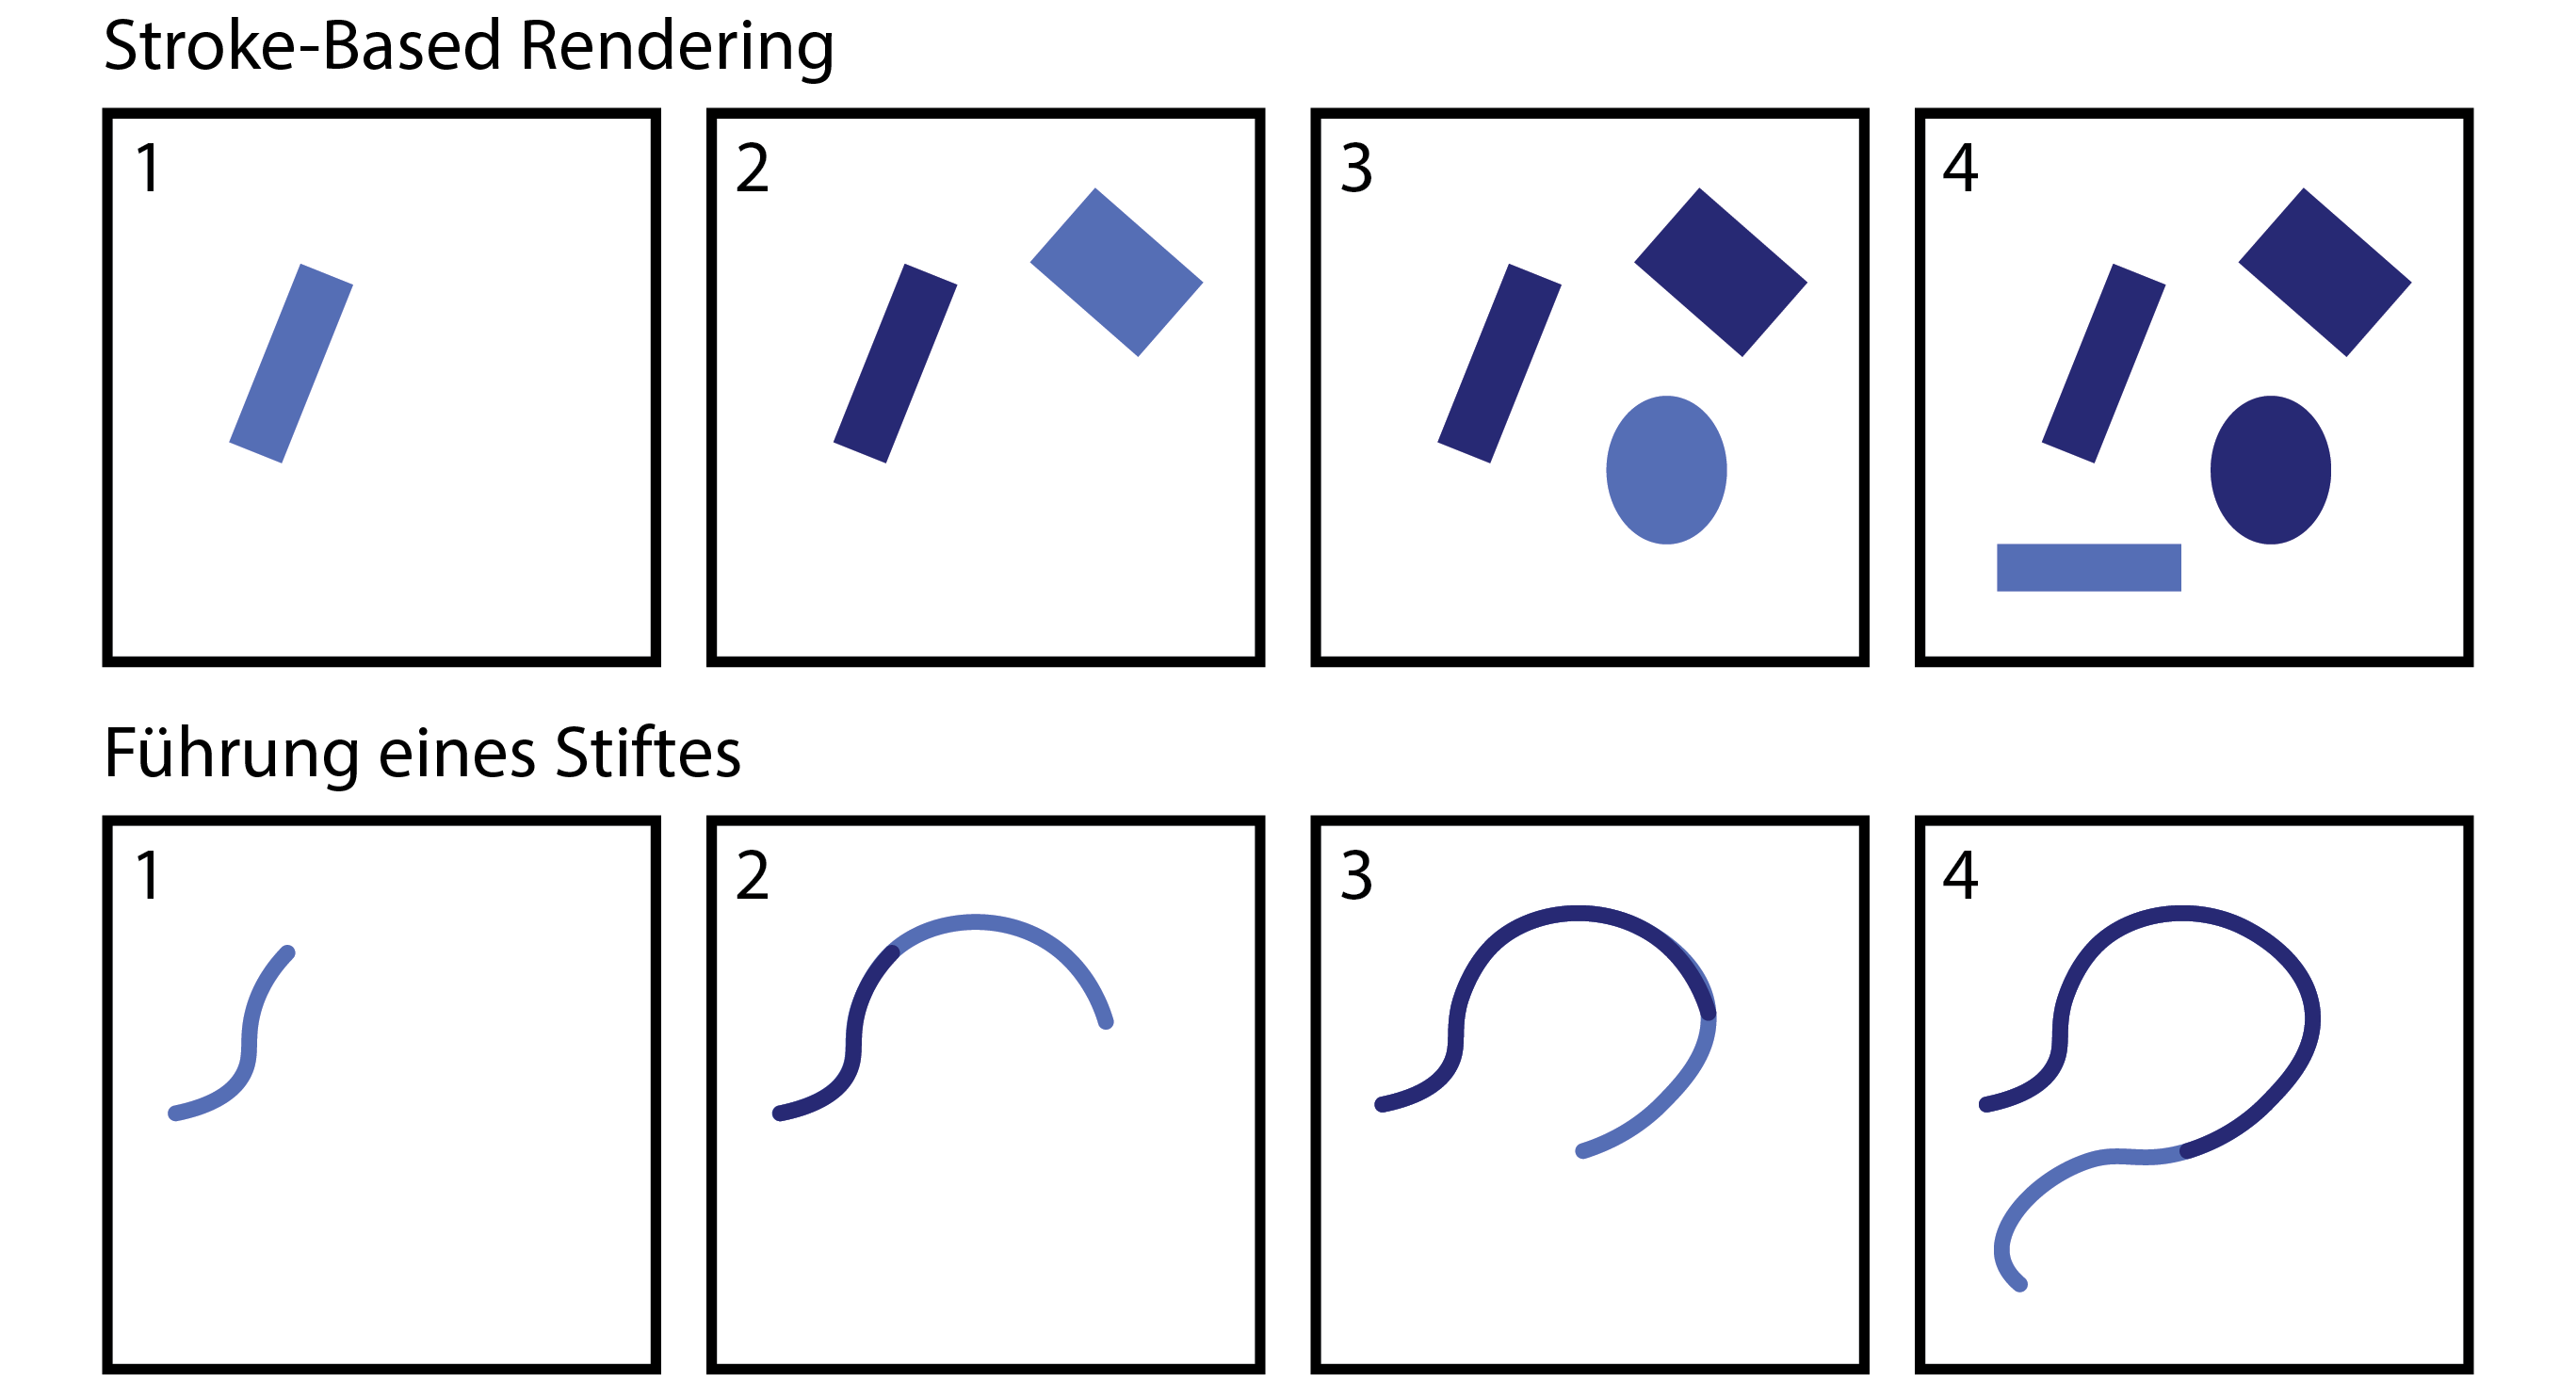
\includegraphics[width=\textwidth]{images/theorie/stroke-v-stift.png}
    \caption{Vergleich zwischen Stroke-Based Rendering und dem Führen eines Stiftes (eigene Abbildung)}
    \label{fig:stroke-v-stift}
\end{figure}
%todo caption, format

\subsection{Doodle-SDQ}\label{sub:t_ver_dood} Doodle-SDQ ist ein
Computerprogramm, das durch ein Reinforcement Learning Modell, spezifischer Deep
Q-Learning (siehe \nameref{sub:t_rl_func}), erlernt, Strichbilder aus dem Google
QuickDraw Datenset \cite{noauthor_quick_2022}
nachzuzeichnen. Nachfolgend sind die Aspekte von Doodle-SDQ beschrieben, die für
diese Arbeit relevant sind.

Die QuickDraw Bilder, die das Programm nachzeichnen soll, sind zu einer
einheitliche Grösse von $84\times84$ Pixeln verarbeiteitet \cite[S.
7]{zhou_learning_2018}. Der Agent kann sich auf einer leeren Zeichenfläche von
der selben Grösse bewegen und zeichnen. Die Umgebung umfasst diese
Zeichenfläche, den Agent und das abzuzeichnende Bild.

Der Agent kann sich durch eine Action in jedem Step auf einen beliebigen Pixel
in einem $11\times11$ Feld, in dessen Zentrum er ist, bewegen. Der Agent kann
ausserdem jede dieser Bewegungen im zeichnenden Zustand oder im nicht
zeichnenden Zustand machen. Der Action-Space hat somit insgesamt eine Grösse von
$2\cdot11\cdot11 = 242$ Actions \cite[S. 5]{zhou_learning_2018}. Im zeichnenden
Zustand wird ein Strich auf der Zeichenfläche zwischen der alten und der neuen
Position des Agenten gezeichnet. Der Agent begeht 100 Steps pro Episode. Eine
neue Episode entspricht dabei einem neuen Bild, das abgezeichnet werden soll.

Die Obervation der Umgebung, und somit der Input in das neuronale Netz (siehe
\nameref{sub:t_rl_func}), ist in zwei Teile gegliedert: den Global Stream und
den Local Stream. Der Global Stream hat eine Form von $28\times28\times4$. Der
Input ist somit dreidimensional. Die Form kann als 4 aufeindandergestapelte
Bilder angesehen werden, die jeweils eine Grösse von $28\times28$ Pixeln haben.
Dabei beschreibt eine relle Zahl den Wert von jedem Pixel in einem Bild. Das
erste Bild im global Stream ist die Vorlage, die abgezeichnet werden soll. Das
zweite Bild ist die Zeichenfläche im aktuellen Zustand. Das dritte Bild
beschreibt die Position des Agents durch seine relative Entfernung zu jedem
Punkt auf der Zeichenfläche. Das vierte Bild beschreibt, ob der Agent im
zeichnenden Zustand ist oder nicht. Wenn alle Pixel dieses letzten Bildes den
Wert $1$ haben, ist der Agent im zeichnenden Zustand. Wenn umgekehrt alle Pixel
den Wert $0$ haben, ist der Agent nicht im zeichnenden Zustand. Der Local Stream
hat eine Form von $11\times11\times2$. Er ist somit auch dreidimensional und
beschreibt zwei gestapelte Bilder. Das erste Bild umfasst die Vorlage in dem
$11\times11$ Bereich (bezeichnet als Local image patch \cite[S.
5]{zhou_learning_2018}), in dem sich der Agent in einem Schritt bewegen kann.
Das zweite Bild beschreibt den selben Bereich von der Zeichenfläche \cite[S. 4
ff.]{zhou_learning_2018}. Der global Stream und der Local Stream werden durch
eine Concatenation Layer (siehe \nameref{sub:t_ml_nn}) zusammengeführt. 

\section{Git und GitHub}\label{chap:t_git} Git und Github sind weit verbreitete
Hilfsmittel für Software Entwickler. Git ist ein Programm, während GitHub ein
Service ist, der dieses Programm in der Cloud zugänglich macht. GitHub hat
zusätzliche Funktionen, die die Zusammenarbeit zwischen mehreren Entwicklern
erleichtern. Die genaue Funktion und das Zusammenspiel dieser beiden Hilfsmittel
wird nachfolgend erläutert.

\subsection{Git}\label{sub:t_git_git} Git erkennt Veränderungen im Code eines
Projektes und speichert diese Veränderungen in einer neuen Version ab. Die
einzelnen Versionen des Projektes bleiben dabei zu jedem Zeitpunkt abrufbar.
Dieses Konzept nennt sich Version Control
\cite{atlassian_git-flow-workflow_nodate}. Das Programm wurde 2005 von Linus
Torvald entwickelt \cite{noauthor_git_2021}. Versionen des Projektes werden
manuell durch einen Commit gespeichert. Es wird empfohlen, nur jeweils ein
bestimmtes Problem oder eine bestimmte Funktion pro Commit anzugehen
\cite{noauthor_5_nodate}. Für grössere Funktionen oder Probleme kann ein Branch
erstellt werden. Ein Branch ermöglicht eine abgekapselte Entwicklung eines
Projektes \cite{guillermo_brachetta_what_2022}. Zum Beispiel kann das Projekt in
mehreren Branches gleichzeitig und unabhängig von einander entwickelt werden
\cite{guillermo_brachetta_what_2022}. Eine weit verbreitete Arbeitsweise und
Branch Struktur mit Git ist GitFlow
\cite{noauthor_what_2022}\cite{atlassian_git-flow-workflow_nodate}. GitFlow
schlägt grundsätzlich einen Main Branch, einen Develop Branch und verschiedene
Feature Branches vor \cite{atlassian_git-flow-workflow_nodate}. Professionelle
Anwendungen von GitFlow verwenden ausserdem so genannte Release Branches und
Hotfix Branches \cite{cameron_mckenzie_gitflow_2021}. Im Main Branch sind
offizielle Versionen des Projektes gespeichert, Im Develop Branch wird das
Projekt als ganzes entwickelt, und in jedem Feature Branch wird eine
Funktionalität in das Projektes implementiert (siehe \autoref{fig:git-branch}). 

% bild branch structure
\begin{figure}[!ht]
    \centering
    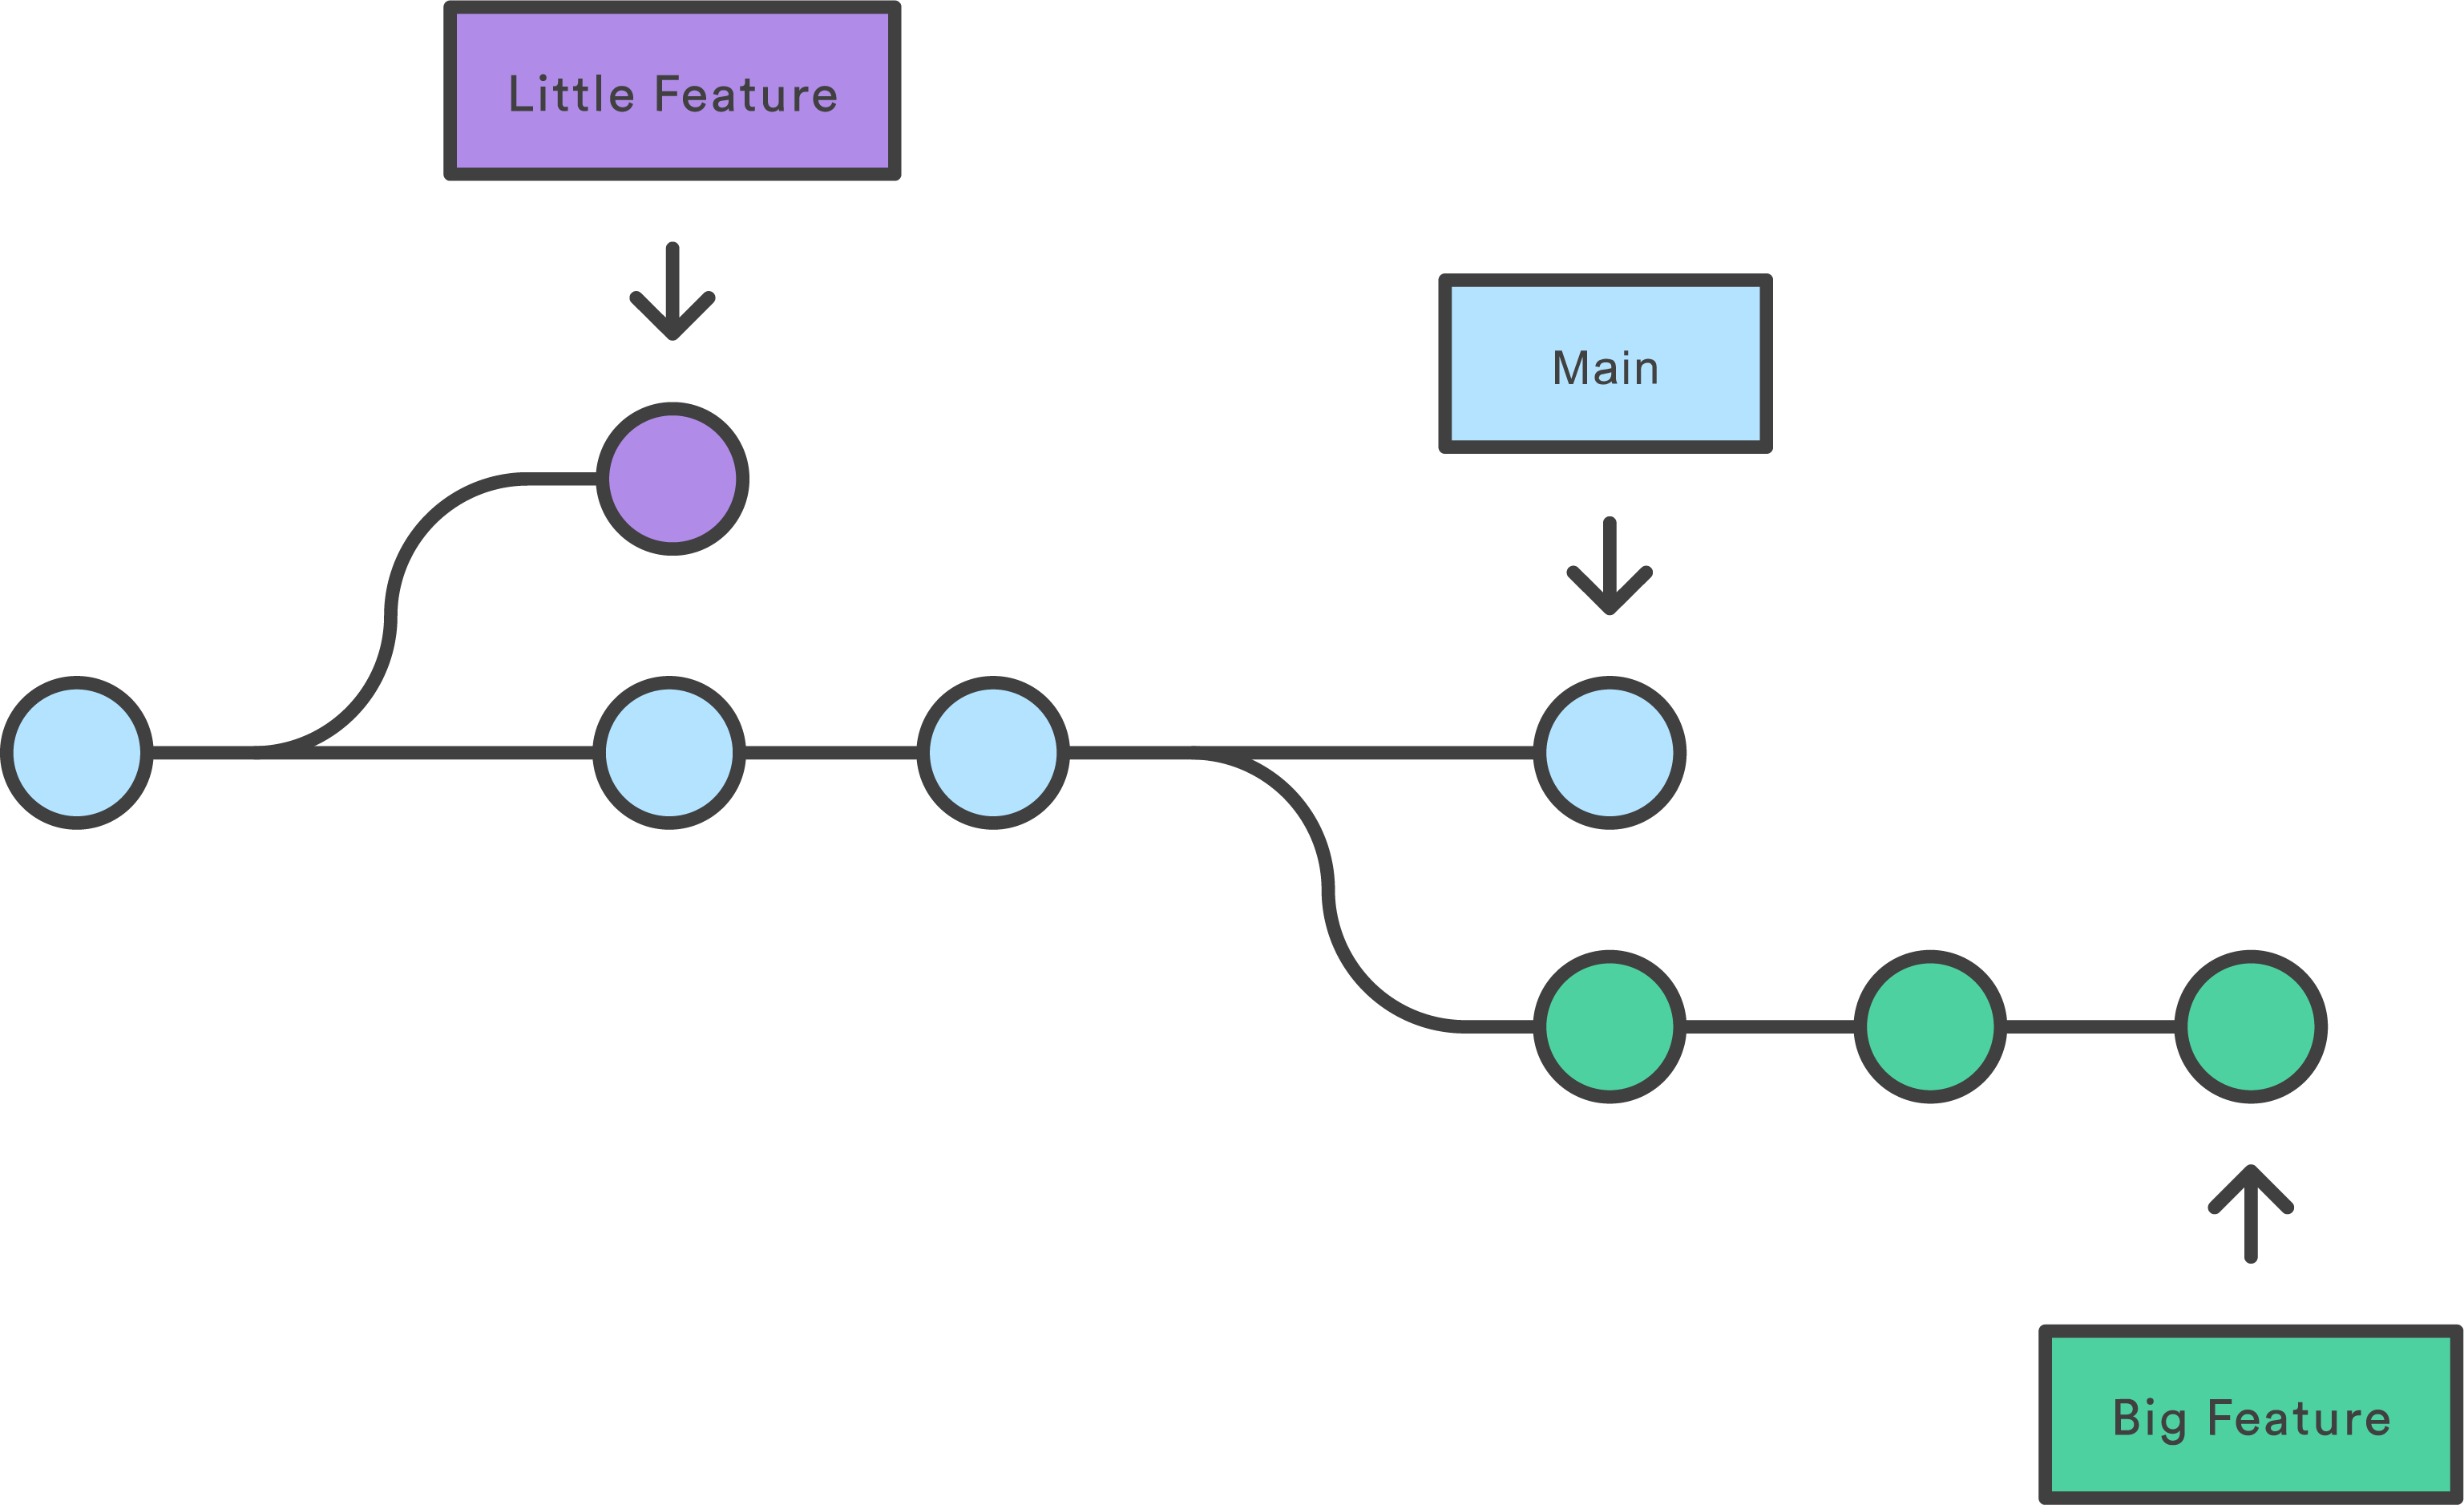
\includegraphics[width=\textwidth-2cm]{images/theorie/git-branch.png}
    \caption{Branch Struktur von GitFlow \cite{atlassian_git-flow-workflow_nodate}}
    \label{fig:git-branch}
\end{figure}
%todo caption, format

\subsection{GitHub}\label{sub:t_git_gh}
GitHub wurde 2008 von Chris Wanstrath, PJ Hyett, Scott Chacon und Tom
Preston-Werner entwickelt \cite{noauthor_github_2021}. 2018 wurde das
Unternehmen von Microsoft gekauft. GitHub ist ein Service, der Projekte, die mit
Git verwalten werden, in der Cloud speichert. Dadurch kann ein Projekt überall
und von beliebig vielen Personen entwickelt werden. GitHub betreibt eine
Webseite, über welche der Service verwendet werden kann
\cite{noauthor_github_2021}.

GitHub besitzt verschiedene Hilfsmittel, die die Zusammenarbeit von Entwicklern
weiter vereinfachen. Beispiele dafür sind Issues und Project Boards. Diese
Hilfsmittel ermöglichen Organisation, Strukturierung und Arbeitsteilung. Ein
weiteres Hilfsmittel sind Pull Requests. Eine Pull Reqeust wird dann gestellt,
wenn die Arbeit an einem Branch fertig ist. Durch Pull Requests können die
Entwickler des Projektes die Funktionalität eines Branches überprüfen. Wenn ein
Branch nicht die gewünschte Aufgabe erfüllt, kann die Pull Request abgelehnt
werden. Erst wenn eine Pull Request angonommen wird, kann der Branch wieder in
den Main Branch zurückgeführt werden \cite{atlassian_pull_nodate}.

